%%%%%%%%%%%%%%%%%%%%%%%%%%%%%%%%%%%%%%%%%%%%%%%%%%%%%%%%%%%%%%%%%
\chapter{BACKGROUND}\label{ch:2_background}
%%%%%%%%%%%%%%%%%%%%%%%%%%%%%%%%%%%%%%%%%%%%%%%%%%%%%%%%%%%%%%%%%
\vspace*{-12pt} % If no text above section, use this vspace* to lift the whole part to the proper starting point - SBÖ
\section{Basic Plasma \& RF Thruster Physics}\label{ChBasicPlasma}
RF ion thruster accelerates charged particles called ions up to 40 km/s to produce thrust\cite{goebel2008fundamentals}. Accelerated ions are sourced from the plasma generated and sustained within the thruster. Before elaborating further on the thruster systems a basic understanding of plasma physics is required. 

\par Plasma is defined as combination of positively charged ions, negatively charged electrons and neutral particles. Densities of charged ions and electrons are assumed equal. This equilibrium state is referred as "quasi-neutrality"\cite{Calik2011}. Thus on a macroscopic scale plasma is considered to be charged neutrally. 
This neutral state is violated under two conditions. One of the conditions is when the plasma is studied near its boundary regions. In such regions due to interaction with the thruster walls a \textit{sheath} is formed in which the densities of positively and negatively charged particles vary.
Second condition occurs when the plasma is examined in microscopic scales. In microscopic scales there are regions in which the neutrality is broken\cite{lieberman2005principles}. The size of such regions are approximated by a certain lenght called \textit{Debye length}.  Effects of plasma sheaths, their occurance and relation to Debye length will be discussed in chapter \ref{ch:sheaths}. 

\par Since plasma has a certain amount of electric charge it can be affected by magnetic and electrical forces\cite{Couch2017}. General behaviour of electric and magnetic fields generated by plasma acts in compliance with Maxwell's equations which are provided in equations \ref{eq:maxwell1} \cite{griffiths2005introduction}.

\begin{equation}
    \begin{aligned}  
    \nabla \cdot \mathbf{E} = \frac{\rho}{\epsilon_0} \\
    \nabla \cdot \mathbf{B} = 0 \\
    \nabla \times \mathbf{E} = - \frac{\partial B}{\partial t} \\
    \nabla \times \mathbf{B} = \mu_0 \left(\textbf{J}+\epsilon_0 \frac{\partial \mathbf{E}}{\partial t}\right)
\end{aligned}
\label{eq:maxwell1}
\end{equation}


In which \textbf{E} is the electric field vector, \textbf{B} is the magnetic flux vector, $\rho$ is the plasma charge density, $\epsilon_0$ and $\mu_0$ are permittivity and permeability of vacuum respectively and \textbf{J} is the current density\cite{goebel2008fundamentals}. Plasma charge density $\rho$ is defined as;
\begin{equation}
    \rho = \sum_{n} q_s n_s = e (Z n_i - n_e)
    \label{eq:plasmacharge}
\end{equation}

where $q_s$ is the charge state and $n_s$ is the number density of an arbitrary species named \textit{s}. e is the electron charge, Z is the charge state, $n_i$ is the ion density, $n_e$ is the electron density. Current charge density \textbf{J} is formulated by the equation\cite{goebel2008fundamentals};

\begin{equation}
    J = \sum_{s} q_s n_s \upsilon_s = e (Z n_i \upsilon_i - n_e \upsilon_e)
    \label{eq:currentchargedensity}
\end{equation}

in which $\upsilon_s$, $\upsilon_i$ and $\upsilon_e$ are the velocities of the species \textit{s}, the ion and the electron, respectively. Electric field \textbf{E} occuring in the ion thrusters is given as\cite{Couch2017};

\begin{equation}
    \mathbf{E} = - \nabla \varPhi 
\end{equation}

where $\varPhi$ is the electric potential.
%  Value of \textbf{E} is negative since \textbf{E} always points in the direction of motion.  

\par Motion of a charged particle within the thruster can be described by equation \ref{eq:lorentz}
\begin{equation}
    \mathbf{F} = m\frac{d\mathbf{v}}{dt} = q(\mathbf{E}+\upsilon \times \mathbf{B})
    \label{eq:lorentz}
\end{equation}

Which is defined as the Lorentz force equation\cite{goebel2008fundamentals}. In the case of magnetic field \textbf{B} in axial direction of the thruster with no electric field \textbf{E} the motion of particles can be found from equation \ref{eq:lorentz}.

\begin{equation}
    \begin{aligned}  
m\frac{\partial v_x}{\partial t} = q B v_y \\
m\frac{\partial v_y}{\partial t} = -q B v_x \\
m\frac{\partial v_z}{\partial t} = 0 \\
\end{aligned}
\label{eq:lorentzxdir}
\end{equation}

Taking one more time derivative of equation \ref{eq:lorentzxdir} results;

\begin{equation}
    \begin{aligned}
        a = \frac{\partial^2 v_x}{\partial t^2} = \frac{qB}{m}\frac{\partial v_y}{\partial t} \\
        a = \frac{\partial^2 v_y}{\partial t^2} = -\frac{qB}{m}\frac{\partial v_x}{\partial t}
    \end{aligned}
    \label{eq:lorentzxdir2}
\end{equation}

Substituting partial time derivative values from equation \ref{eq:lorentzxdir} into equation \ref{eq:lorentzxdir2} yields;

\begin{equation}
    \begin{aligned}
        \frac{\partial^2 v_x}{\partial t^2} = - \left(\frac{qB}{m}\right)^2 v_x \\
        \frac{\partial^2 v_y}{\partial t^2} = - \left(\frac{qB}{m}\right)^2 v_y
    \end{aligned}
    \label{eq:lorentxdir3}
\end{equation}

Equation \ref{eq:lorentxdir3} shows that particle displays a harmonic oscillation with a certain frequency defined as cyclotron frequency $\omega_c$;

\begin{equation}
    \omega_c = \frac{qB}{m}
    \label{eq:cyclotronfreq}
\end{equation}


% Reassembling the equations at equation \ref{eq:lorentzxdir} gives

% \begin{equation}
%     \frac{m}{qB}\frac{\partial v_x}{\partial t} = v_y
% \end{equation}

% The part $\dfrac{qB}{m}$ is defined as cyclotron frequency and denoted as $w_c$.

% Integrating the equation \ref{eq:lorentzxdir} once for velocity and twice for position vectors yield\cite{lara2016design};

% \begin{equation}
%     \begin{aligned}
%         v_x = \frac{q}{|q|}v_n sin(w_c t + \varphi ) \\
%         v_y = -\frac{q}{|q|}v_n cos(w_c t + \varphi)
%     \end{aligned}
%     \label{eq:velvectors}
% \end{equation}

% \begin{equation}
%     \begin{aligned}
%         x = \frac{v_n}{w_c}cos(w_c t + \varphi) \\
%         y = \frac{v_n}{w_c}sin(w_c t + \varphi) \\
%     \end{aligned}
%     \label{eq:posvectors}
% \end{equation}

% From equations \ref{eq:velvectors} and \ref{eq:posvectors} it can be seen that the particle performs a circular motion within the magnetic field with a constant velocity $v_n$ and cyclotron frequency $w_c$.
 Orbit size of this circular motion can be found by observing this circular motion displayed in figure \ref{fig:larmor}.

\begin{figure}[ht]
    \centering
    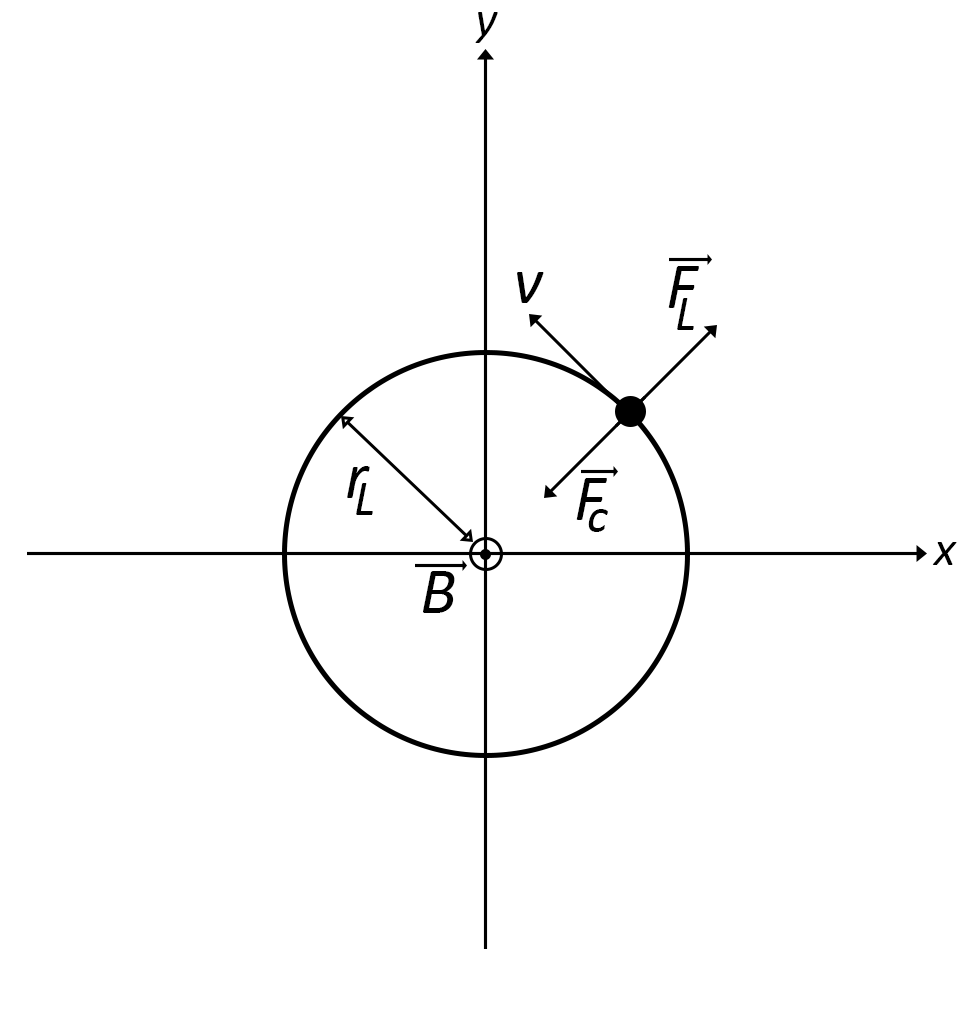
\includegraphics[scale=0.25]{fig/larmor.png}
    \caption{Motion of a particle in a uniform axial magnetic field}
    % {Motion of a particle in a uniform axial magnetic field\cite{lara2016design}}
    \label{fig:larmor}
\end{figure}

Charged particle shown in figure \ref{fig:larmor} will act under the influence of a Lorentz force;
\begin{equation}
    \mathbf{F} = q\mathbf{v} \times \mathbf{B}
    \label{eq:circularlorentz}
\end{equation}

Same particle will also feel a centripetal force;
\begin{equation}
    \mathbf{F_c} = \frac{mv^2}{r_L}
    \label{eq:centripetal}
\end{equation}

For a constant uniform motion equations \ref{eq:circularlorentz} and \ref{eq:centripetal} must be equal.

\begin{equation}
    q\mathbf{v} \times \mathbf{B} = \frac{mv^2}{r_L}
    \label{eq:larmor}
\end{equation}

where $r_L$ is the \textit{Larmor radius} and is the radius of the particle's circular motions shown in equation \ref{eq:larmorradi}
\begin{equation}
    r_L = \dfrac{mv}{qB}
    \label{eq:larmorradi}
\end{equation}


% Same magnetic field \textbf{B} also creates an electric field \textbf{E}. Direction of this electric field is perpendicular to the magnetic field. If the direction of the magnetic field is assumed as axial then the electric field direction becomes tangential. 

% \par There are different types of plasma that occur on low pressure enviroment; DC glow discharge, capacitively coupled plasma(CCP) and inductively coupled plasma(ICP)


% \begin{equation}

%     \label{eq:lorentzydir}
% \end{equation}

% \begin{equation}

%     \label{eq:lorentzzdir}
% \end{equation}

% where $\upsilon$ is particle velocity and \textbf{F} is thrust. Since energetic electrons inside the ion thruster act mainly under the influence of the electric field other elements of equation \ref{eq:lorentz} can be omitted\cite{goebel2008fundamentals}. Rewriting equation \ref{eq:lorentz} can simply be rewritten;

% \begin{equation}
%     \mathbf{F} = q\mathbf{E}
%     \label{eq:lorentzsimple}
% \end{equation}

% Assuming a Maxwellian distribution among the particles average three dimensional kinetic energy and particle speed equations can be expressed as\cite{griffiths2005introduction};

% \begin{equation}
%     E_{avg} = \frac{3}{2}kT
% \end{equation}

% \begin{equation}
%     \overline{\upsilon} = \sqrt{\left(\frac{2kT}{\pi m}\right)}
% \end{equation}

% where m is the mass of particle, k is Boltzmann's constant and T is the temperature. 

\subsection{Sheats at The Boundaries of The Plasma} \label{ch:sheaths}

Earlier in the chapter \ref{ChBasicPlasma} it was mentioned that the quasi-neutral stance of the plasma is broken along the plasma boundary in regions called sheaths. Since ion acceleration grids exploit the sheath at the edge of the plasma a solid understanding of sheath behavior is very important to model and design an ion thruster.

After the initial ignition of plasma created ions and free electrons will be lost due to interaction with the containing walls. Since electrons have much higher velocities compared to ions they will exit the plasma in larger quantities. Over time this imbalance creates a negatively biased container walls with respect to the plasma. This negative charge attracts ions from the plasma and repel the electrons, causing a non-neutral region on the border of plasma. This region in which the plasma loses its neutrality is called sheath\cite{lara2016design}.

\begin{figure}[ht]
    \centering
    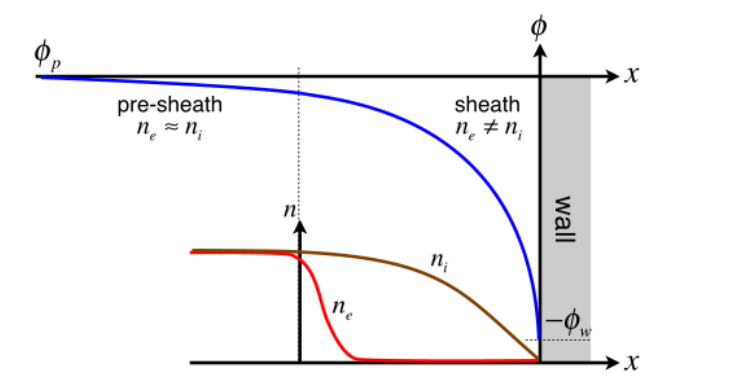
\includegraphics[scale=0.75]{fig/sheath.png}
    \caption[Potential and species density change near plasma boundary]{Potential and species density change near plasma boundary\cite{lara2016design}}
    \label{fig:sheathgraph}
\end{figure}
\newpage
Figure \ref{fig:sheathgraph} shows how the species densities and potential is changing while approaching the plasma boundary. As particles get close to the wall negative potential $-\phi_w$ attracts ions and repels electrons causing a charge inbalance. The thickness of this sheath region is given in the order of Debye lenght $\lambda_D$\cite{goebel2008fundamentals}. Thanks to the shield that occurs the remainder of plasma maintains its potential $\phi_p$. 

% If the potential throughout the sheath is too large compared to the electron temperature a sheath forms. If this potential is large enough the electrons are repelled away from the plasma. Under these circumstances the electron density in the regions around the sheath edge is close to zero. 

% \begin{equation}
%     J = \frac{4 \epsilon_0}{9}\sqrt{\frac{2e}{M}}\frac{V^{\frac{3}{2}}}{l_e^2}
%     \label{eq:childlangmuir}
% \end{equation}

% The result gives J, current density or current per unit area. In equation \ref{eq:childlangmuir} M is the mass of the particle, V is the voltage and $l_e$ is the sheath thickness which can be calculated by using the following formula\cite{williams2013ion};

% \begin{equation}
%     l_e = \sqrt{(l_g + t_s)^2+\frac{d_s^2}{4}}
%     \label{eq:sheaththickness}
% \end{equation}

% where $l_g$ is the distance between grids, $t_s$ is the screen grid thickness and $d_s$ is the diameter of one aperture of the screen grid. Representations of the same parameters can also be seen in figure \ref{fig:sheaththickness}.
% \newpage

% \begin{figure}[ht]
%     \centering
%     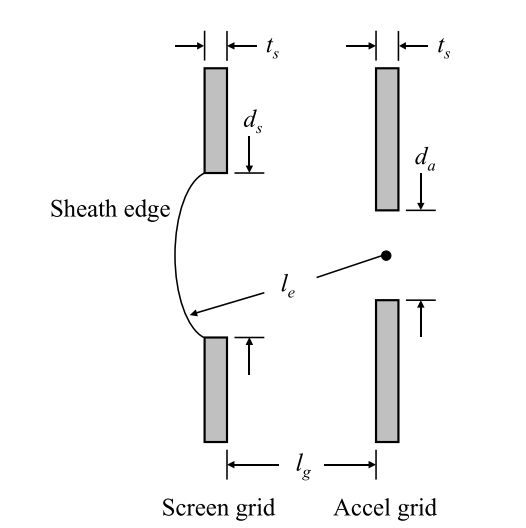
\includegraphics[scale=0.75]{fig/sheaththickness_toddwilliams.png}
%     \caption[Sheath forming representation between grids]{Sheath forming representation between grids\cite{williams2013ion}}
%     \label{fig:sheaththickness}
% \end{figure}




% \section{Rocket Equation For RF Ion Thrusters}

\section{General RF Ion Thruster Design Parameters} \label{ch:generaldesign}

General design of RF ion thruster was shown in figure \ref{fig:rfschematic}. This figure will be examined by dividing the figure into two main regions. One of these regions is where the plasma ignition occurs and the other is where the ion extraction and ejection are performed. \\
Within the thruster the plasma is ignited and sustained within the discharge chamber.  Propellant is fed into the discharge chamber. Plasma is then created by means of an RF coil wrapped around the discharge chamber. An RF signal is put through this coil creates an electromagnetic field within the discharge chamber and ignites the plasma. During operation coil does not come into contact with the plasma. Both RF coil and the discharge chamber constitute the plasma ignition region.
Created quasi-neutral plasma interacts with a pair of grids placed at the exit of the discharge chamber. This pair of grids make up the ion extraction and ejection region. By oppositely polarizing the grids an electrostatic field is created which extract and ejects the ions. \\
Parameters regarding the design of discharge chamber, RF coil and ion extraction grids affect the thrust and specific impulse values of the thrusters. They will be examined individually in the following subsections. 
\subsection{Discharge Chamber and RF Coil}

Plasma is created and sustained in discharge chamber. As a result most of plasma-surface interaction occurs within the discharge chamber. Energetic particles, both ions and electrons, are
lost to the discharge chamber walls. Initial RF ion thruster designs included cylindrical discharge chambers in order to ease the RF coil placement. An example of this cylindirical design can be seen in figure \ref{fig:RIT2}. 
\newpage
\begin{figure}[ht]
    \centering
    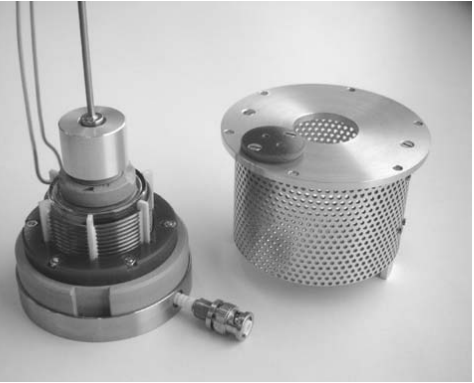
\includegraphics[scale=0.8]{fig/RIT2.png}
    \caption[Disassembled model of RIT-2 developed by Giessen University]{Disassembled model of RIT-2 developed by Giessen University\cite{loeb2004development}}
    \label{fig:RIT2}
\end{figure}

In the figure \ref{fig:RIT2} discharge chamber is shown at the left side, wrapped by a coil. Length of the coil depends on the length of the discharge chamber. If the discharge chamber is long 
then more antenna can be accomodated which in turn creates more induction. But as a downside longer discharge chamber means longer particle loss area for the plasma. Research have been conducted to reduce the particle loss area without drastically altering the coil. As a result conical and hemispherical discharge chambers have been devised. Examples for conical and hemispherical discharge chamber designs can be seen in figures \ref{fig:RITXT} and \ref{fig:RIT45} respectively

\begin{figure}[ht]
    \centering
    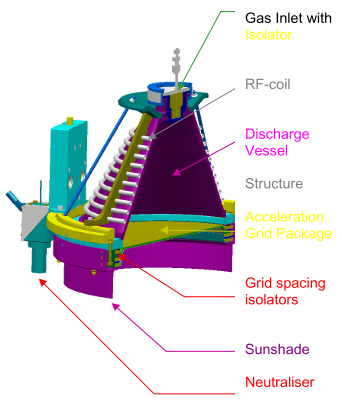
\includegraphics[scale=0.75]{fig/RITXT.png}
    \caption[Cutaway drawing of RIT-XT thruster highlighting conical design]{Cutaway drawing of RIT-XT thruster highlighting conical design\cite{leiter2003development}}
    \label{fig:RITXT}
\end{figure}
\newpage
\begin{figure}[ht]
    \centering
    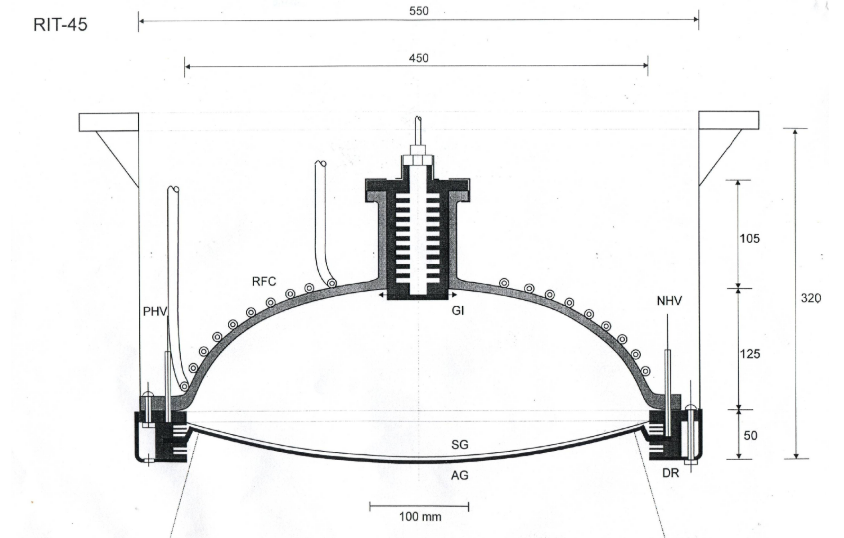
\includegraphics[scale=.6]{fig/RIT45.png}
    \caption[Hemispherical discharge chamber schematic of RIT-45]{Hemispherical discharge chamber schematic of RIT-45\cite{loeb2011design}}
    \label{fig:RIT45}
\end{figure}

Since RF coil is located at the outside of the discharge chamber, RF signals have to be able to easily penetrate the chamber walls in order to form electromagnetic fields inside the chamber. Since an electrical conductive material would act as a Faraday cage and keep RF signals from penetrating, the material of discharge chamber has to be non-conductive. Non-conductive and thermally durable materials such as quartz or alumuna have been common choices for discharge chamber material\cite{goebel2008fundamentals}. \\
RF coil is made of a highly conductive material such as copper. An example of RF coil is shown in figure \ref{fig:coppercoil}

\begin{figure}[ht]
    \centering
    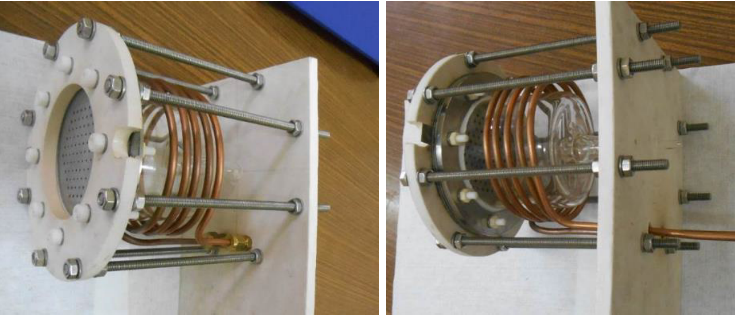
\includegraphics[scale=.75]{fig/burfitcoil.png}
    \caption[Copper coil wrapped around BURFIT-80 thruster]{Copper coil wrapped around BURFIT-80 thruster\cite{kokal2017design}}
    \label{fig:coppercoil}
\end{figure}
\newpage

Another RF antenna configuration is planar antenna. In this configuration RF antenna is placed at the base of discharge chamber as shown in figure \ref{fig:planarantenna}.
\begin{figure}[ht]
    \centering
    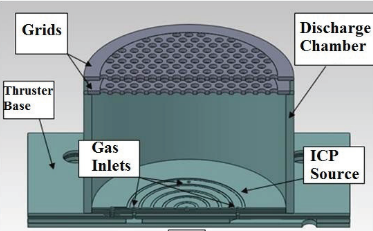
\includegraphics{fig/planarantenna.png}
    \caption[Planar antenna, denoted as ICP source, placed at the base of discharge chamber]{Planar antenna, denoted as ICP source, placed at the base of discharge chamber\cite{Bumbarger}}
\label{fig:planarantenna}
\end{figure}

Planar antenna configuration results in high-density and more uniform plasma discharge compared to wrapped RF coil configurations. This configuration is ideal since the area around the 
discharge chamber remains empty and can accomodate other optional thruster elements such as magnets for plasma containment. Since focus of this work is simplicity and scalability of ion thrusters there 
will be no magnets present. This situation also negates the need for a planar RF antenna configuration\cite{gillman2008low}. 

Frequency of broadcasted signal through RF coil is important.  Literature survey reveals that for optimal power transfer from coil to plasma, broadcasted signal frequency should be half of particle collision frequency\cite{holste2018performance}. In typical thrusters RF frequency is kept in the order of 1MHz\cite{goebel2008analytical}. In this work however RF signal frequency will be 13.56 MHz which is an industrial-scientific-medical standard. RF power supply that will be used in this work is originally designed for industrial processes such as plasma etching. For this work the power supply will be repurposed to fit RF ion thruster operations. 

Inductivity of the coil is directly related to the number of turns it makes around the discharge chamber. High turn number means higher inductivity however it also means longer coil. Longer coil will waste more power due to ohmic losses\cite{tsay2012micro}. In order to reach an optimal level a trade-off has to be made. 

\subsection{Ion Extraction Grids}
Ion extraction is performed by a group of aligned grids. They are placed in tandem to each other as shown in the schematic at figure \ref{fig:rfschematic}. Grid located closer to the plasma is named \textit{screen} grid whereas the grid located away from the plasma is called \textit{accelerator} grid. These grids contain numerous apertures in them as shown in figures \ref{fig:burfitscreen} and \ref{fig:burfitscreen}. 

\begin{figure}[ht]
    \centering
    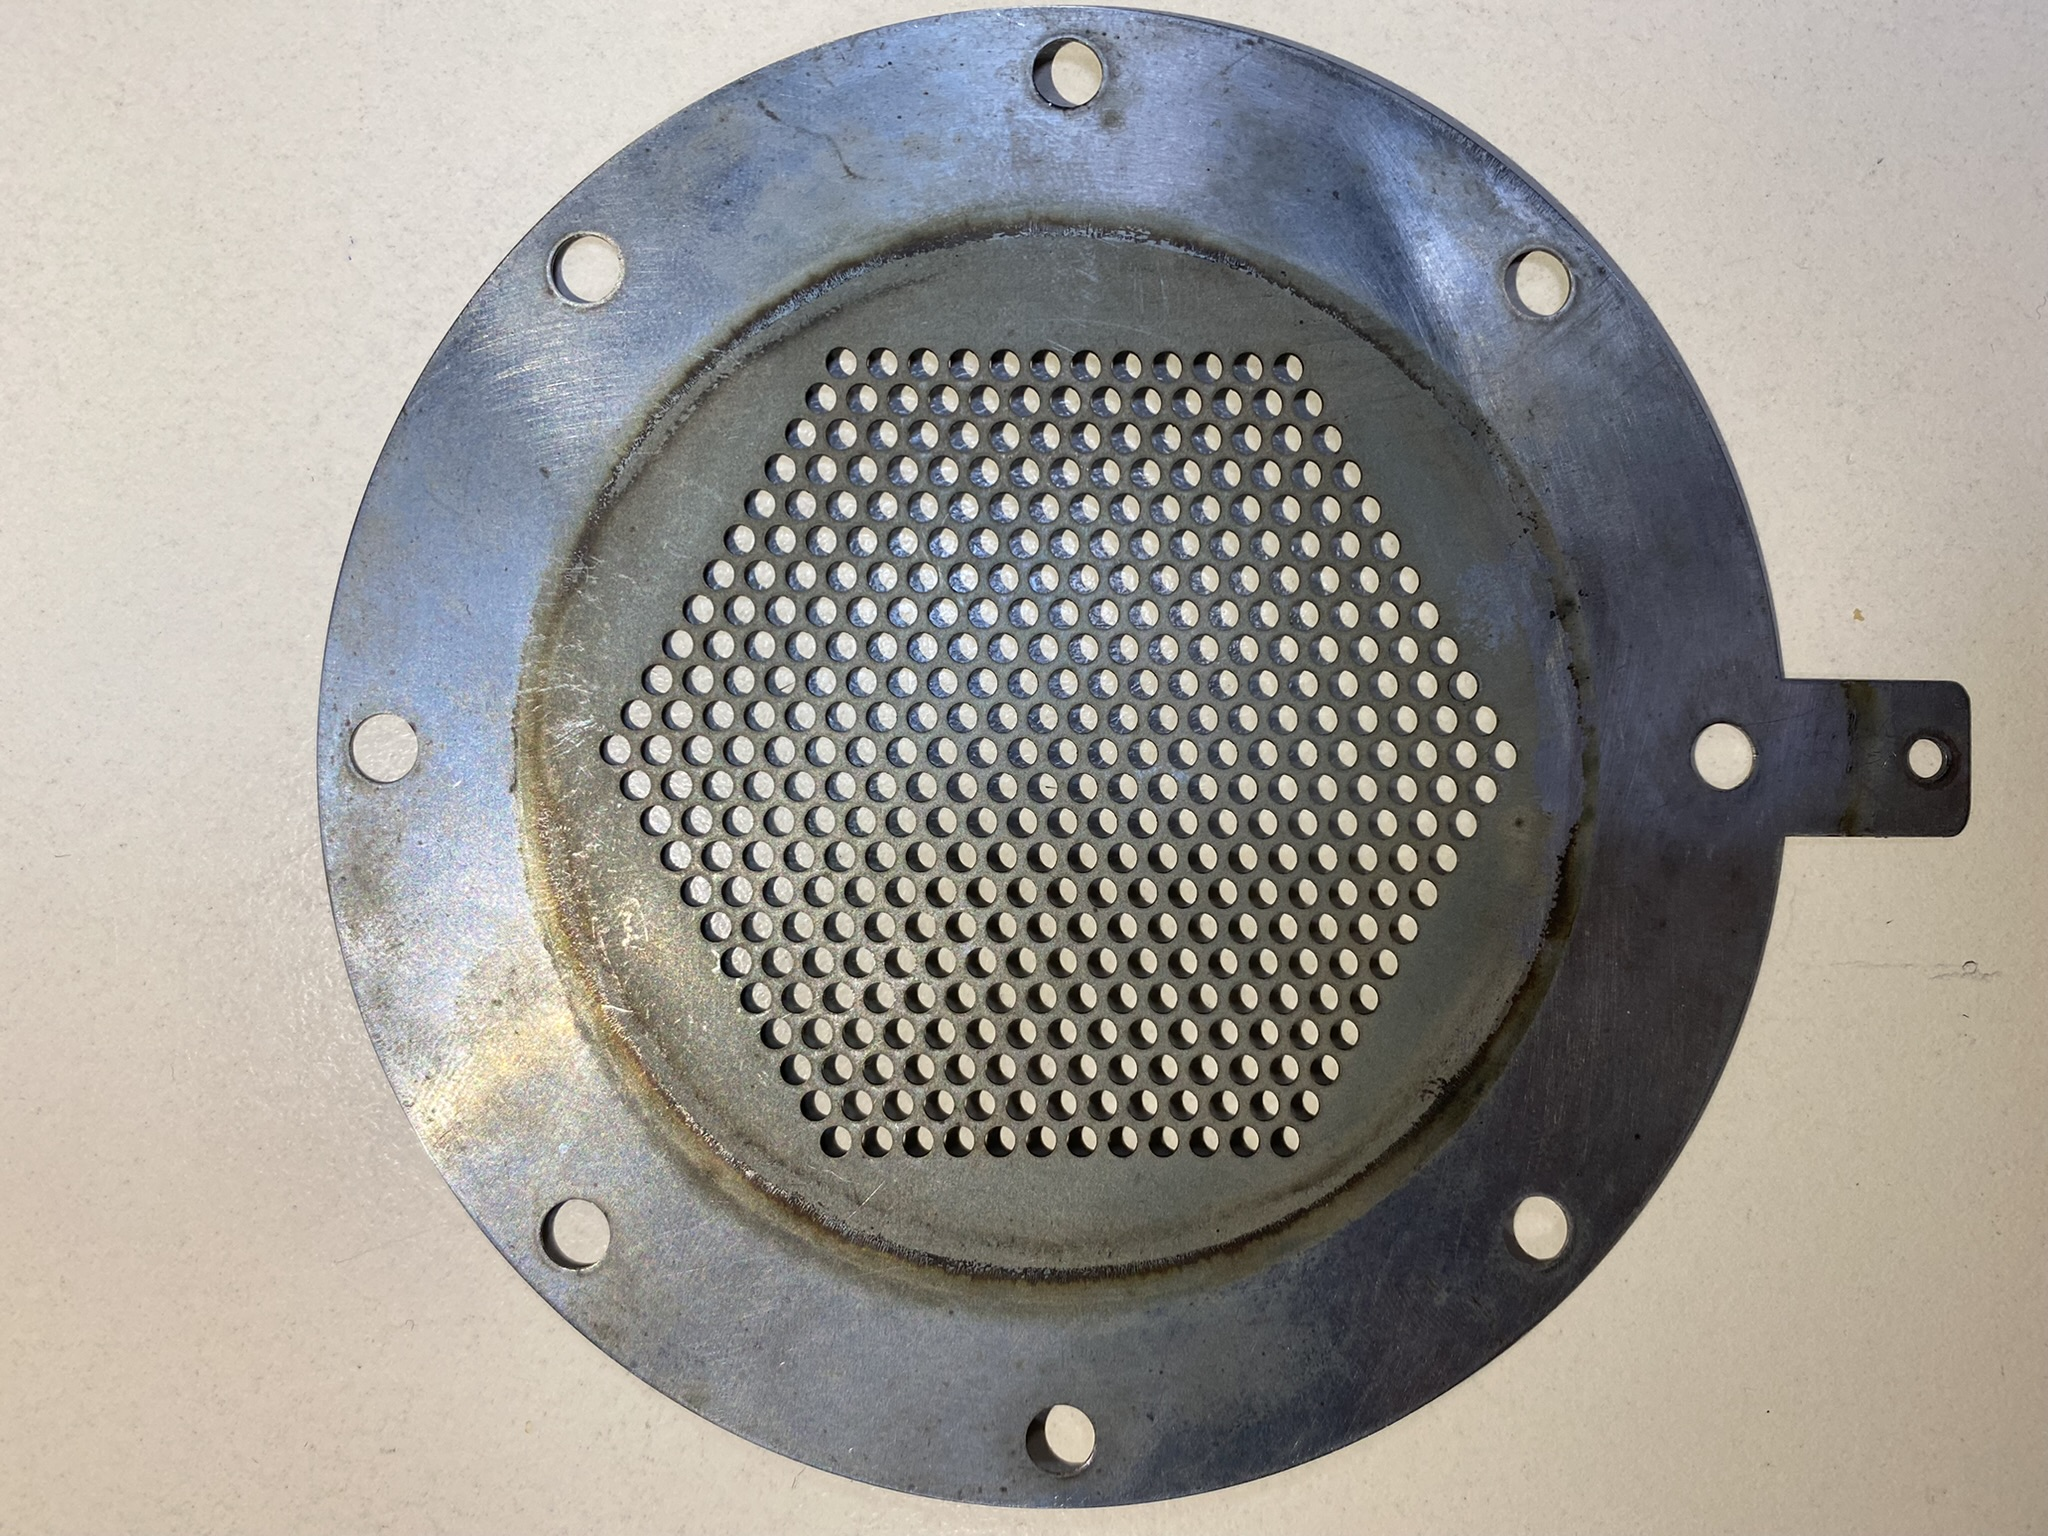
\includegraphics[scale=0.15]{fig/screen.jpeg}
    \caption{Screen grid of BURFIT-80}
    \label{fig:burfitscreen}
\end{figure}
\newpage
\begin{figure}[ht]
    \centering
    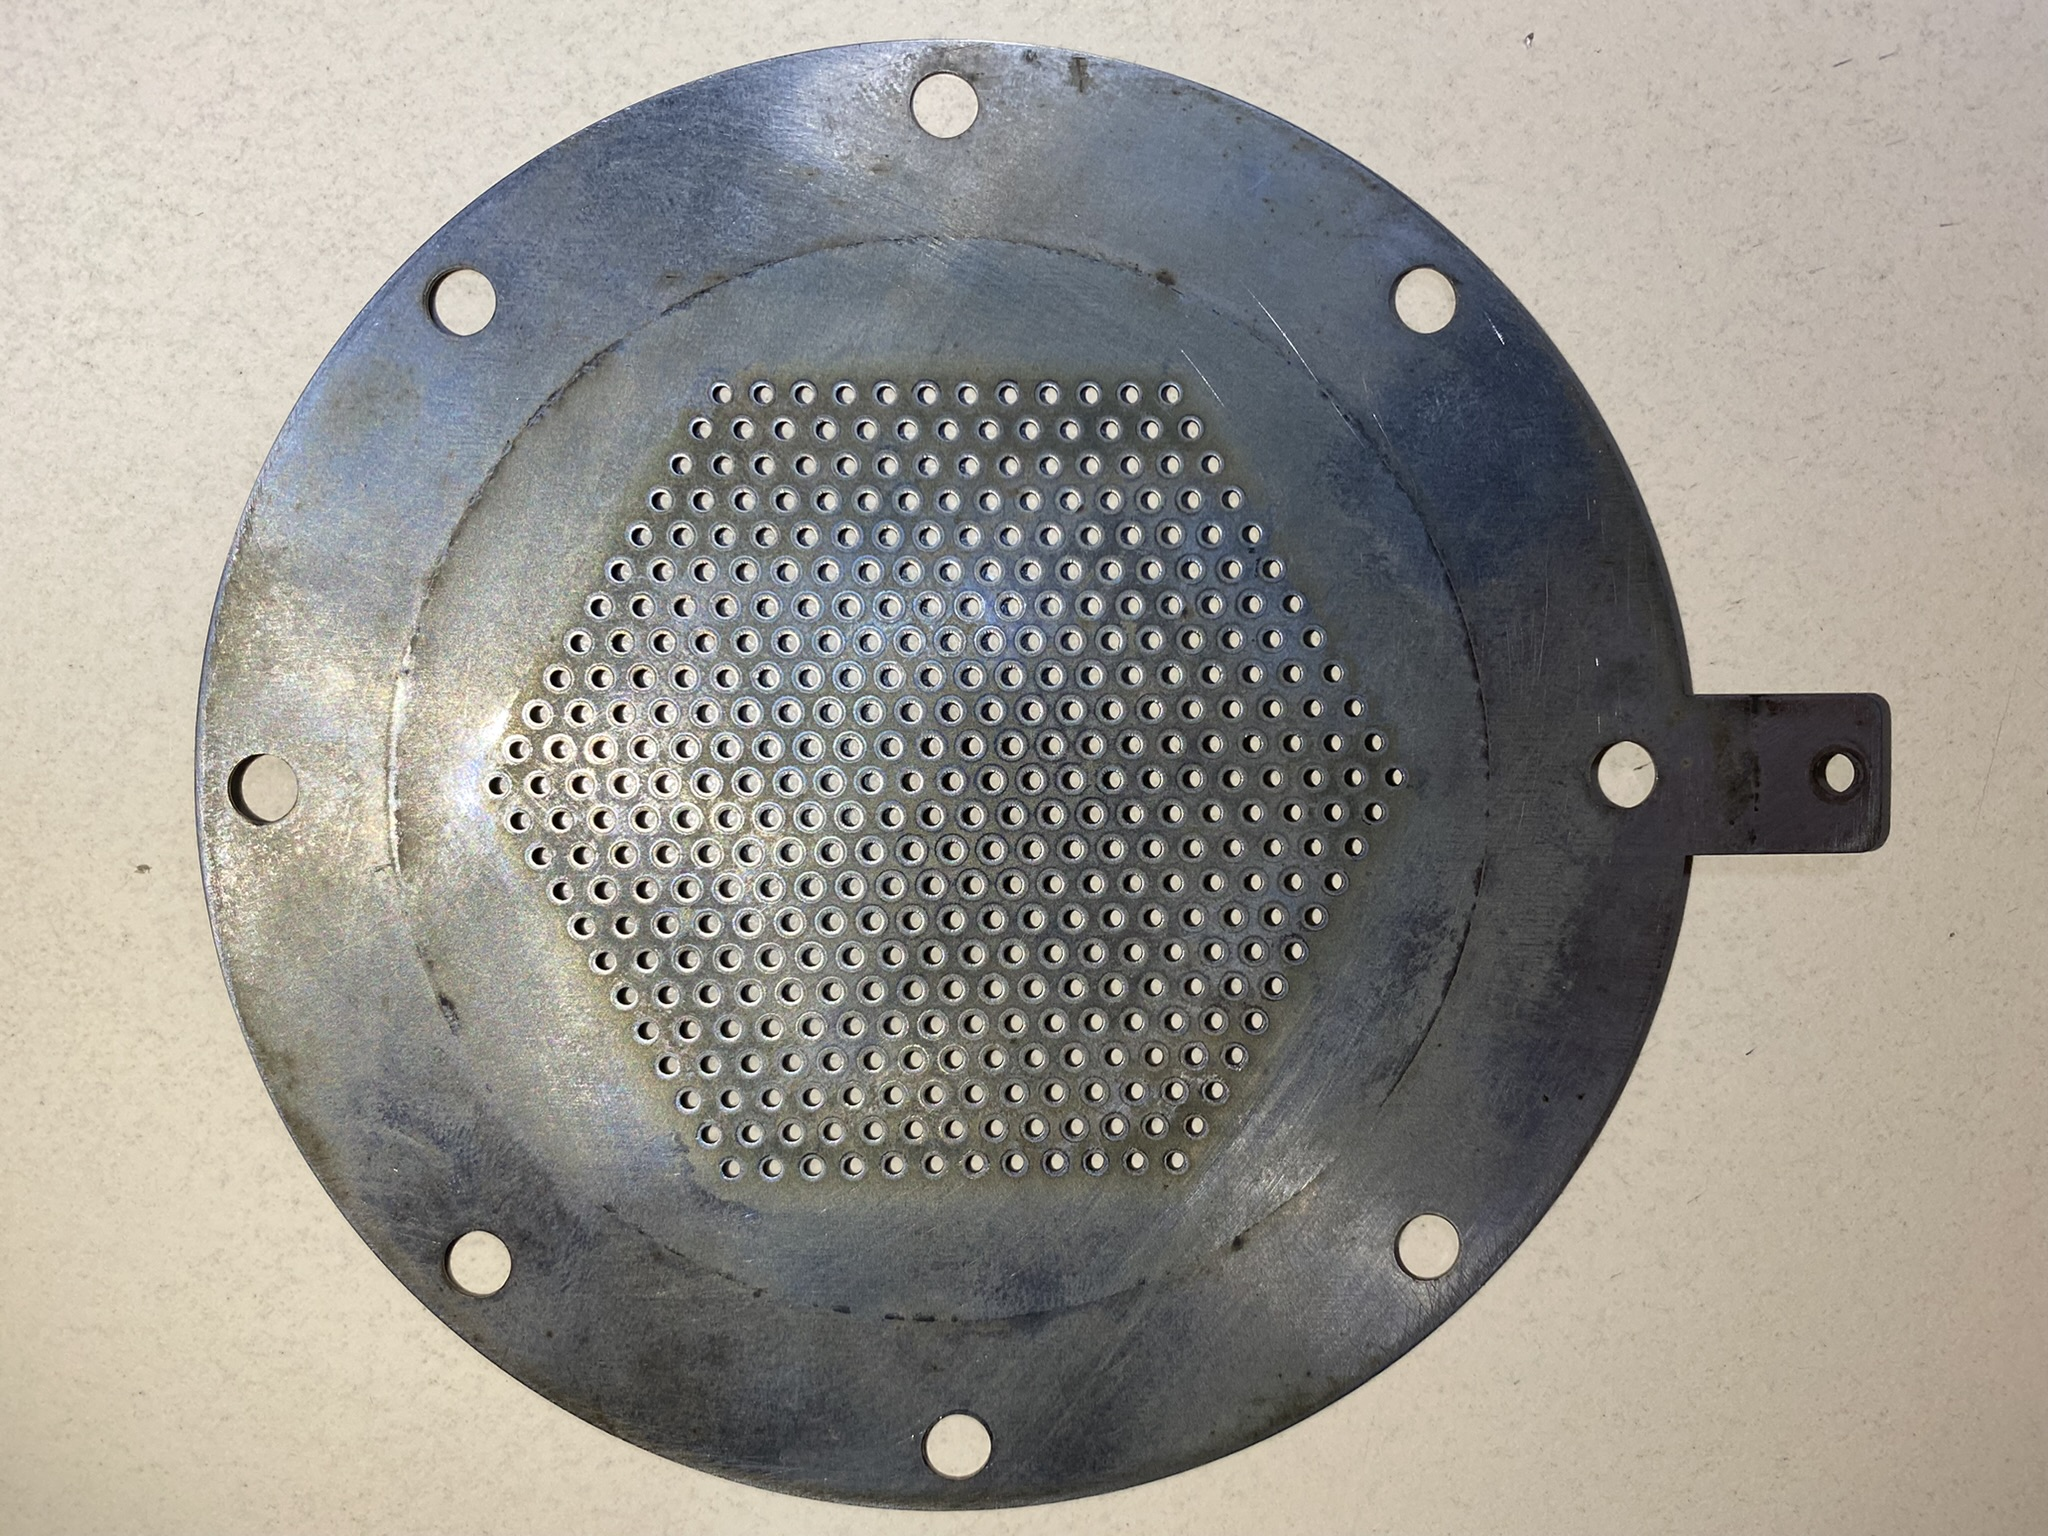
\includegraphics[scale=0.15]{fig/accel.jpeg}
    \caption{Accelerator grid of BURFIT-80}
    \label{fig:burfitaccel}
\end{figure}

When oppositely biased, grids create an electrostatic field and exploit the plasma sheath that forms at the intersection of plasma and grid surfaces.
 Accelerator grid is negatively biased in order to attract positively charged ions in the plasma. When directly exposed to plasma high speed collisions between ions and accelerator grid cause sputtering and erode the grid, effectively reducing its lifetime. In order to shield the accelerator grid and properly channel the ion flow, screen grid is used. When located in between the accelerator grid and biased positively, screen grid forces ions to channel through the grids. Potential variations of grids is shown in graph at figure \ref{fig:potvariation}.
 Biasing voltages for screen grid and accel grid are in the range of +200V and -1000V respectively. 
\newpage
 \begin{figure}[ht]
     \centering
     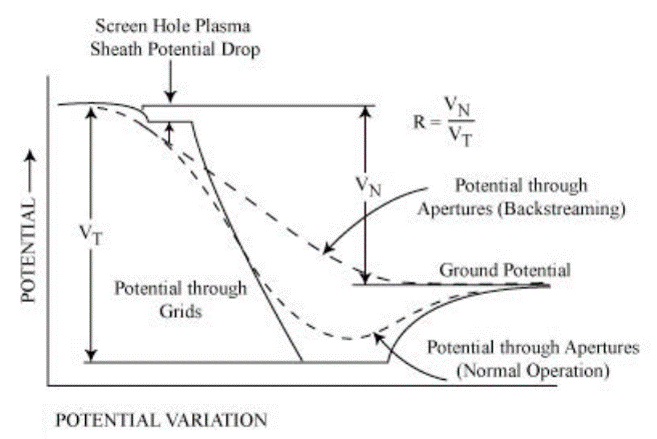
\includegraphics[scale=0.9]{fig/potvariation.png}
     \caption[Grid Potential Variations]{Grid Potential Variations\cite{OCW1964}}
     \label{fig:potvariation}
 \end{figure}
  
 In order to ensure robust channeling of ions through the grids the screen and accelerator grids need to be properly aligned and distanced. Diameters of apertures in grids are also determined accordingly. Diameter of screen grid apertures are generally larger than that of accelerator grid apertures. When grids are properly aligned and ion flow is optimal then grid structure reaches its optimum perveance levels as shown in figure \ref{fig:ionflow}

\begin{figure}[ht]
    \centering
    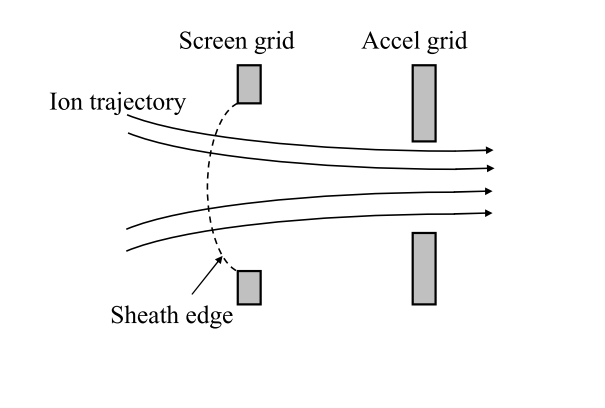
\includegraphics[scale=0.6]{fig/ionflow.png}
    \caption[Ion flow through screen and accelerator grids]{Ion flow through screen and accelerator grids\cite{williams2013ion}}
    \label{fig:ionflow}
\end{figure}

In the event of grid misalignment ion trajectory may display undesirable behaviours such as under-perveance or over-perveance. 
\begin{figure}[ht]
    \centering
    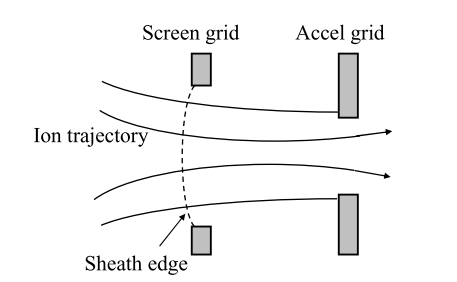
\includegraphics[scale=0.6]{fig/overperveance.png}
    \caption[Over-perveance trajectory of ions]{Overperveance trajectory of ions\cite{williams2013ion}}
    \label{fig:overperveance}
\end{figure}

Figure \ref{fig:overperveance} displays a situation called overperveance in which over focusing ions cause increased ion sputtering on the grids.

\begin{figure}[ht]
    \centering
    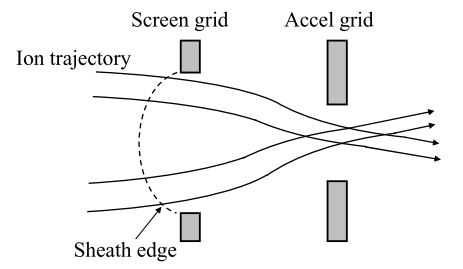
\includegraphics[scale=0.6]{fig/underperveance.png}
    \caption[Under-perveance trajectory of ions]{Overperveance trajectory of ions\cite{williams2013ion}}
    \label{fig:underperveance}
\end{figure}


Another misalignment type occurs when the ions are insufficiently focused in which case ions display a motion shown in figure \ref{fig:underperveance}. This behavior is referred as under-perveance. 

Proper ion flow is dominated by grid aperture and distance parameters shown in figure \ref{fig:gridparams}.
\newpage
\begin{figure}[ht]
    \centering
    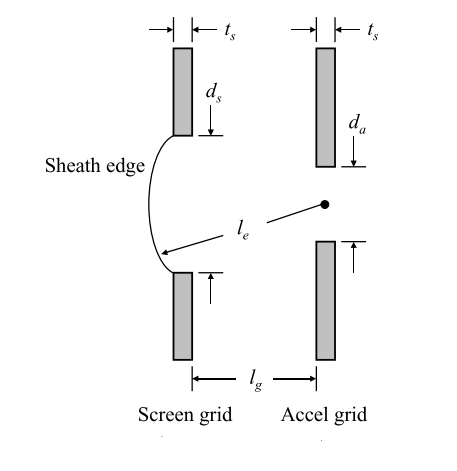
\includegraphics[scale=0.6]{fig/gridparameters.png}
    \caption[Grid structure parameters]{Grid structure parameters\cite{williams2013ion}}
    \label{fig:gridparams}
\end{figure}

In figure \ref{fig:ionflow} $d_s$ and $d_a$ are screen grid aperture and accelerator grid aperture diameter respectively. $l_g$ is the distance between grids. $t_s$ and $t_a$ are thickness of screen and accelerator grid, respectively. Finally, $l_e$ is the effective ion acceleration distance. 

Upon exiting the thrusters ions form beamlets which occur at the downstream direction of grid apertures. Afterwards beamlets mix together and form one continuous ion beam. However occasionally positively charged accelerated ions may backstream towards similarly positively biased accelerator. Ion beamlets, forming of ion beam and backstreaming ions are illustrated in figure \ref{fig:ionbackstream}.

\begin{figure}[ht]
    \centering
    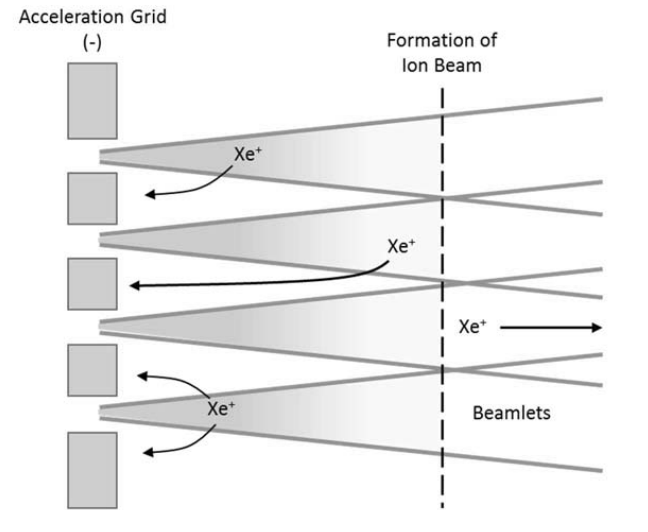
\includegraphics[scale=0.6]{fig/ionbackstream.png}
    \caption[Ion beamlets, beam and escaping ions]{Ion beamlets, beam and escaping ions\cite{Couch2017}}
    \label{fig:ionbackstream}
\end{figure}
Over time collisions between backstreaming ions and accelerator grid can cause erosion significantly reduce the grid's ability to channel ions properly. In order to avoid damage to accelerator grid an additional grid, named \textit{decelerator} grid, can be placed in the downstream direction of ion beam. Decelerator grid is kept at ground potential and shields the accelerator grid from high energy impacts. Placement and working principle of decelerator grid is shown in figure \ref{fig:ionbackstreamdecel}

\begin{figure}[ht]
    \centering
    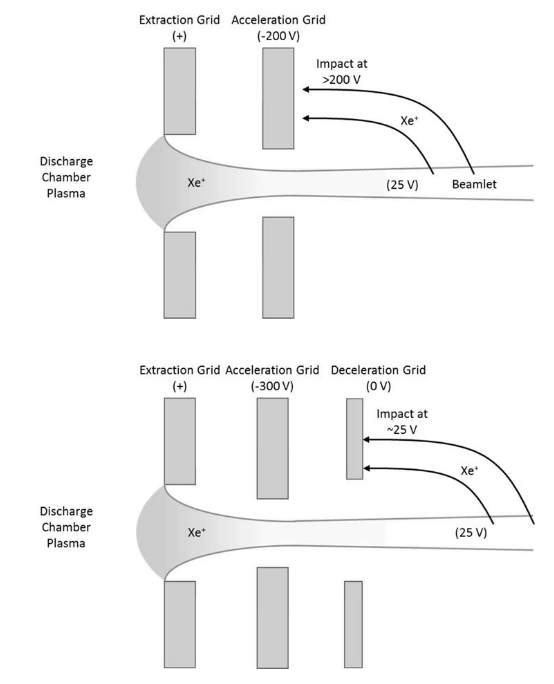
\includegraphics[scale=0.75]{fig/ionbackstreamdecel.png}
    \caption[Comparison of Two and Three Grid Designs]{Comparison of Two and Three Grid Designs\cite{Couch2017}}
    \label{fig:ionbackstreamdecel}
\end{figure}

Electric field vector between grids is in the direction of ion flow; from screen to accelerator grid as shown in figure \ref{fig:gridpot}. 

\begin{figure}[ht]
    \centering
    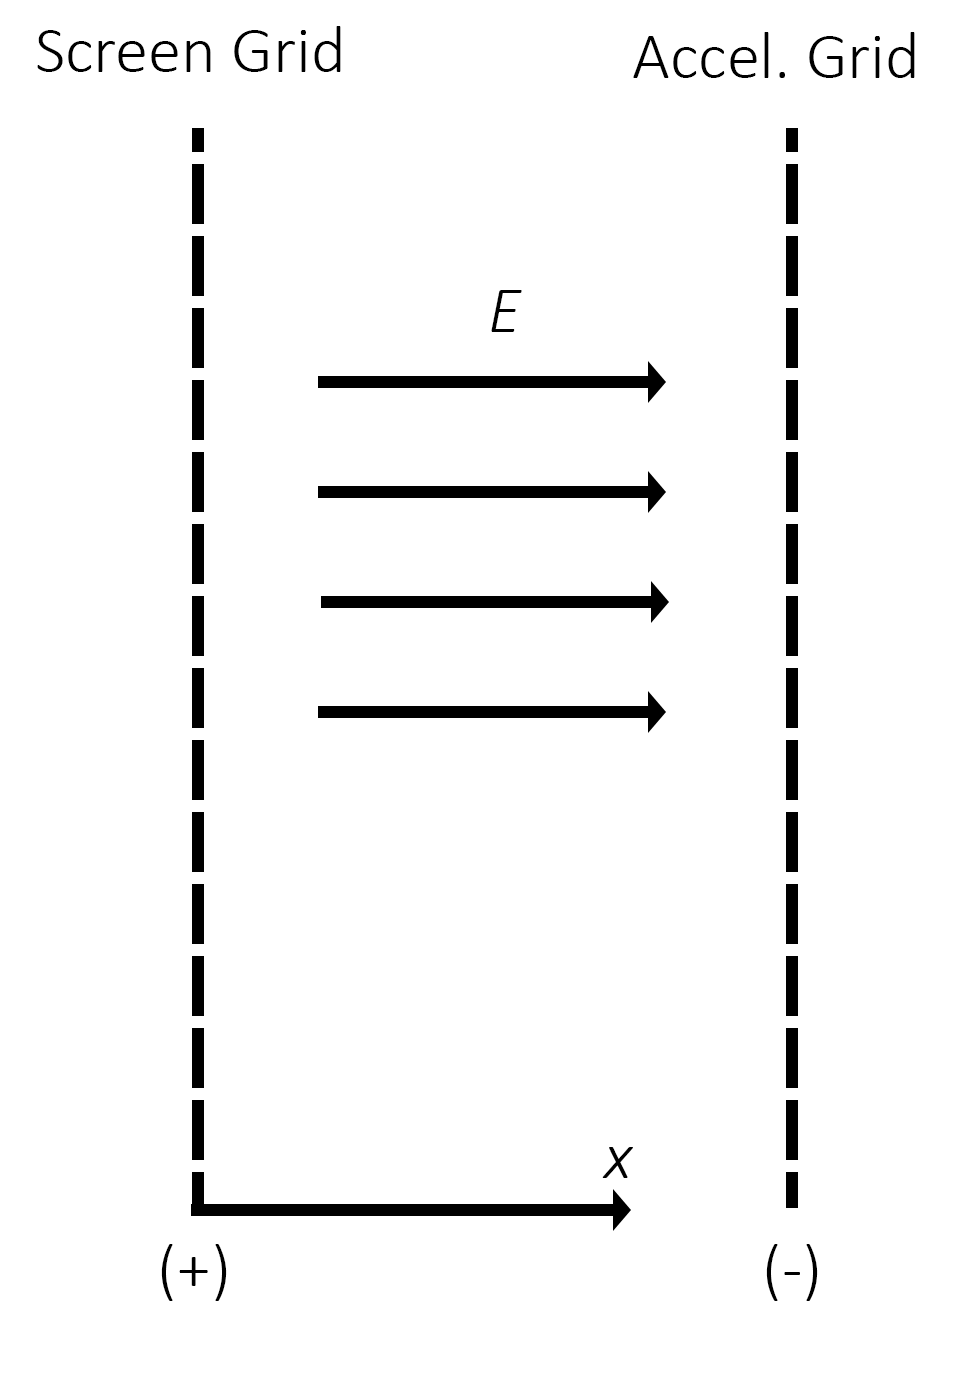
\includegraphics[scale=0.3]{fig/gridpot.png}
    \caption{Electric field vector between grids}
    \label{fig:gridpot}
\end{figure}
\newpage

Within the gap in between grids, Poisson's equation holds\cite{OCW1964};

\begin{equation}
    \frac{d^2\phi}{dx^2} = -\frac{e n_i}{\varepsilon_0}
    \label{eq:poisson}
\end{equation}

where $e$ is the electric charge and $n_i$ is the number of ions. Together, $e n_i$ constitutes $\rho$, charge density. Ion continuity between grids is constant;

\begin{equation}
    j = e n_i v_i
    \label{eq:ioncont}
\end{equation}

where $v_i$ is ion velocity due to electrostatic free-fall.

Particles in the gap is subjected to force $F=qE$.
\begin{equation}
   F =  qE = -e \frac{d \phi}{dx} = m_i \frac{dv}{dt}
    \label{eq:gapforce}
\end{equation}

Multiplying all sides with $dx$ gives;

\begin{equation}
    -ed\phi = m_i\frac{dx}{dt}dv = m_i v dv
    \label{eq:dv}
\end{equation}

\begin{eqnarray}
    ed\phi + m_i v dv = 0
    \label{eq:eq0}
\end{eqnarray}

Taking the integral of \ref{eq:eq0};

\begin{equation}
    e\phi + \frac{1}{2}m_i v^2_i = e\phi_0 + \frac{1}{2}m_i v^2_0
    \label{eq:integrated}
\end{equation}

\begin{equation}
    v^2_i - v^2_0 = \frac{2e(\phi_0 - \phi)}{m_i}
\end{equation}

Assuming inital speeds of ions are negligible;

\begin{equation}
    v_i = \sqrt{\frac{2e(\phi_0 - \phi)}{m_i}}
    \label{eq:ionvel}
\end{equation}


Plugging equations \ref{eq:ioncont} and \ref{eq:ionvel} into equation \ref{eq:poisson} gives 2nd order nonlinear differential equation for electic field between gaps where the potential $\phi$ is known;

\begin{equation}
    \frac{d^2 \phi}{d x^2} + \frac{j}{\varepsilon_0}\sqrt{\frac{m_i}{2e (\phi_0-\phi)}} = 0
    \label{eq:2ndorder}
\end{equation}

Rearranging and integrating equation \ref{eq:2ndorder} gives $E$;

\begin{equation}
    E^2 = \left(\frac{d\phi}{dx}\right)^2 - \left(\frac{d\phi}{dx}\right)^2_{x=0}  = \frac{4j}{\varepsilon_0}\sqrt{\frac{m_i (\phi_0 -\phi)}{2e}}
    \label{eq:integratedE}
\end{equation}

where boundary conditions are\cite{OCW1964};

\begin{equation}
    \begin{aligned}
        \phi(0) = 0 \\
        \phi(x=d) = -V_T
    \end{aligned}
    \label{eq:boundary1}
\end{equation}

where $d$ is the distance between grids and $V_T$ is the accel. grid potential. 

Furthermore another fundamental boundary condition imposed\cite{OCW1964};

\begin{equation}
    \left(\frac{d\phi}{dx}\right)_{x=0}
    \label{eq:boundary2}
\end{equation}

Which can be imposed due to "space charge limitation". When there is no ion flow electric field between grids is constant and dependent on the potentials of screen and accel. grids. As the ions flow from screen to accel. grid electric field is altered. There comes a point where accelerating field near the first grid is cancelled by the downstream of positively charged ions. At this point the grids are accelerating highest current density possible and is space charge limited\cite{lara2016design}. 

\begin{equation}
    E = \frac{d\phi}{dx} \left(\frac{4j}{\varepsilon_0}\right)^{\frac{1}{2}}\left(\frac{m_i (\phi_0 - \phi)}{2e}\right)^{\frac{1}{2}}
\end{equation}

Integrating;

\begin{equation}
    \phi_{x=d} - \phi_{x=0} = - \left[\frac{3}{2}\left(\frac{j}{\varepsilon_0}\right)^{\frac{1}{2}}\left(\frac{m_i}{2e}\right)^{\frac{1}{4}}x\right]^{\frac{4}{3}}\bigg| ^{x=d}_{x=0}
\end{equation}

Substituting boundary conditions from equations \ref{eq:boundary1} and \ref{eq:boundary2} and rearranging gives;

\begin{equation}
    J = \frac{4}{9}\varepsilon_0 \sqrt{\frac{2e}{m_i}}\frac{V_T^{\frac{3}{2}}}{d^2}
    \label{eq:childlangmuir}
\end{equation}

Equation \ref{eq:childlangmuir} gives maximum current density extracted from polarized grids and is referred as Child-Langmuir's Law in which J is current per unit area, $m_i$ is mass of ions, $V_T$ is voltage and $d$ is the sheath thickness.. In order to Relation of Child-Langmuir's Law and thrust calculations will be examined in subsection \ref{ch:subsecthrust}.

Grid structure is constantly in contact with plasma and ions throughout the lifetime of the thruster and thus subjected to heating. In order to preserve grid alignment, grid materials should be chosen from materials with low heat expension coefficient. Additionally chosen material should also exhibit low secondary electron yield\cite{Bumbarger}. In practice grids are generally manufactured from molybdenum, titanium, INVAR or even carbon composite materials\cite{yavuz2013prototype}.
% \subsection{RF Coil}
\subsection{Thrust} \label{ch:subsecthrust}
Thrust is created by accelerating positively charged ions to high velocities and ejecting them from the thruster. Momentum transfer between ions and thruster occurs within accelerator grids thus thrust can be defined by sum of forces applied on screen and accelerator grids\cite{Couch2017} as shown in equations \ref{eq:gridforce} and \ref{eq:gridforcesum}.

\begin{equation}
    \begin{aligned}
        F_{screen} = \frac{1}{2}\epsilon_0 E^2_{screen} \\
        F_{accel} = -\frac{1}{2}\epsilon_0 E^2_{accel} 
    \end{aligned}
\label{eq:gridforce}
\end{equation}

\begin{equation}
    F = F_{screen} + F_{accel} = \frac{1}{2}\epsilon_0 (E^2_{screen}-E^2_{accel})
    \label{eq:gridforcesum}
\end{equation}

Thrust calculations can also be performed by evaluating the momentum change with respect to time;

\begin{equation}
T = \frac{d}{dt}(mv) = \frac{d}{dt}(m_p v_{ex}) =  \dot{m}_p v_{ex}    
\label{eq:momentumchange}
\end{equation}

where $\dot{m}_p$ is the propellant flow rate and $v_{ex}$ is the exhaust velocity. Equation \ref{eq:momentumchange} is same for all thruster systems. Specifically for electric propulsion systems it can be refined as;

\begin{equation}
    T = \dot{m}_p v_{ex} \sim \dot{m}_i v_i
    \label{eq:epthrust}
\end{equation}

Since ion thrusters achieve most of its thrust from ejected ions, propellant mass and exhaust velocity in equation \ref{eq:momentumchange} can be exchanged with ion mass flow rate 
$\dot{m}_i$ and ion velocity $v_i$\cite{goebel2008fundamentals}.

Electric energy is converted into kinetic energy in the thruster.

\begin{equation}
    \frac{1}{2}m_i v_i = e V_b
    \label{eq:kineticenergy}
\end{equation}

Where $V_b$ is the ion beam potential. From equation \ref{eq:kineticenergy} ion velocity $v_i$ can be defined as;

\begin{equation}
    v_i = \sqrt{\frac{2eV_b}{m_i}}
    \label{eq:ionvel2}
\end{equation}

Ion beam current, $I_b$, for fully and singly ionized propellant is defined as\cite{goebel2008fundamentals};

\begin{equation}
    I_b = \dot{m}_i\left(\frac{e}{m_i}\right)
    \label{eq:ionbeamcurrent}
\end{equation}

Substituting equations \ref{eq:ionvel2} and \ref{eq:ionbeamcurrent} into equation \ref{eq:epthrust} gives the thrust formula;

\begin{equation}
    T = \sqrt{\frac{2 m_i V_b}{e}} I_b
    \label{eq:uncorrectedthrust}
\end{equation}

Thrust defined in equation \ref{eq:uncorrectedthrust} is applicable for ideal conditions only. Unideal conditions during thruster operations warrant the inclusion  of additional correction factors. 

One of the unideal conditions is ion beam divergence. Ions contribute to thrust only when they are moving in the opposite direction of spacecraft velocity vector. Other ions diverting from this direction do not provide thrust and are considered as loss. 

\begin{figure}[ht]
    \centering
    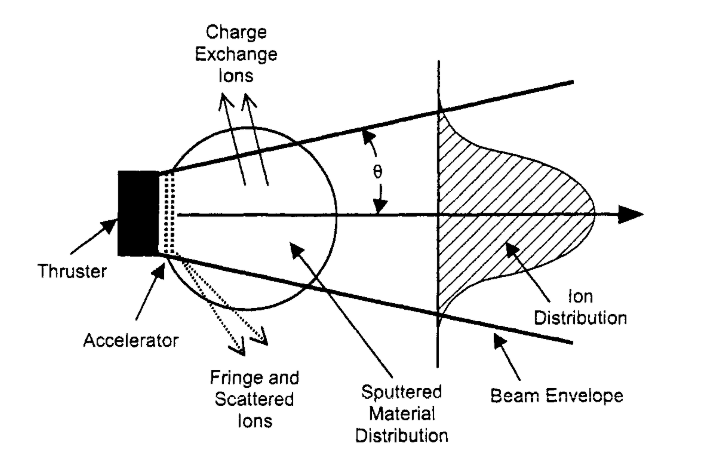
\includegraphics[scale=.75]{fig/beamdivergence.png}
    \caption[Beam plume behaviour after exiting thruster]{Beam plume behaviour after exiting thruster\cite{goebel2008fundamentals}}
    \label{fig:beamdivergence}
\end{figure}

In the figure \ref{fig:beamdivergence}, angle $\theta$ is defined as half-angle of ion beam divergence. It can also be observed in figure \ref{fig:beamdivergence2} which was taken during when BURFIT-80 thruster was operating. 

\begin{figure}[ht]
    \centering
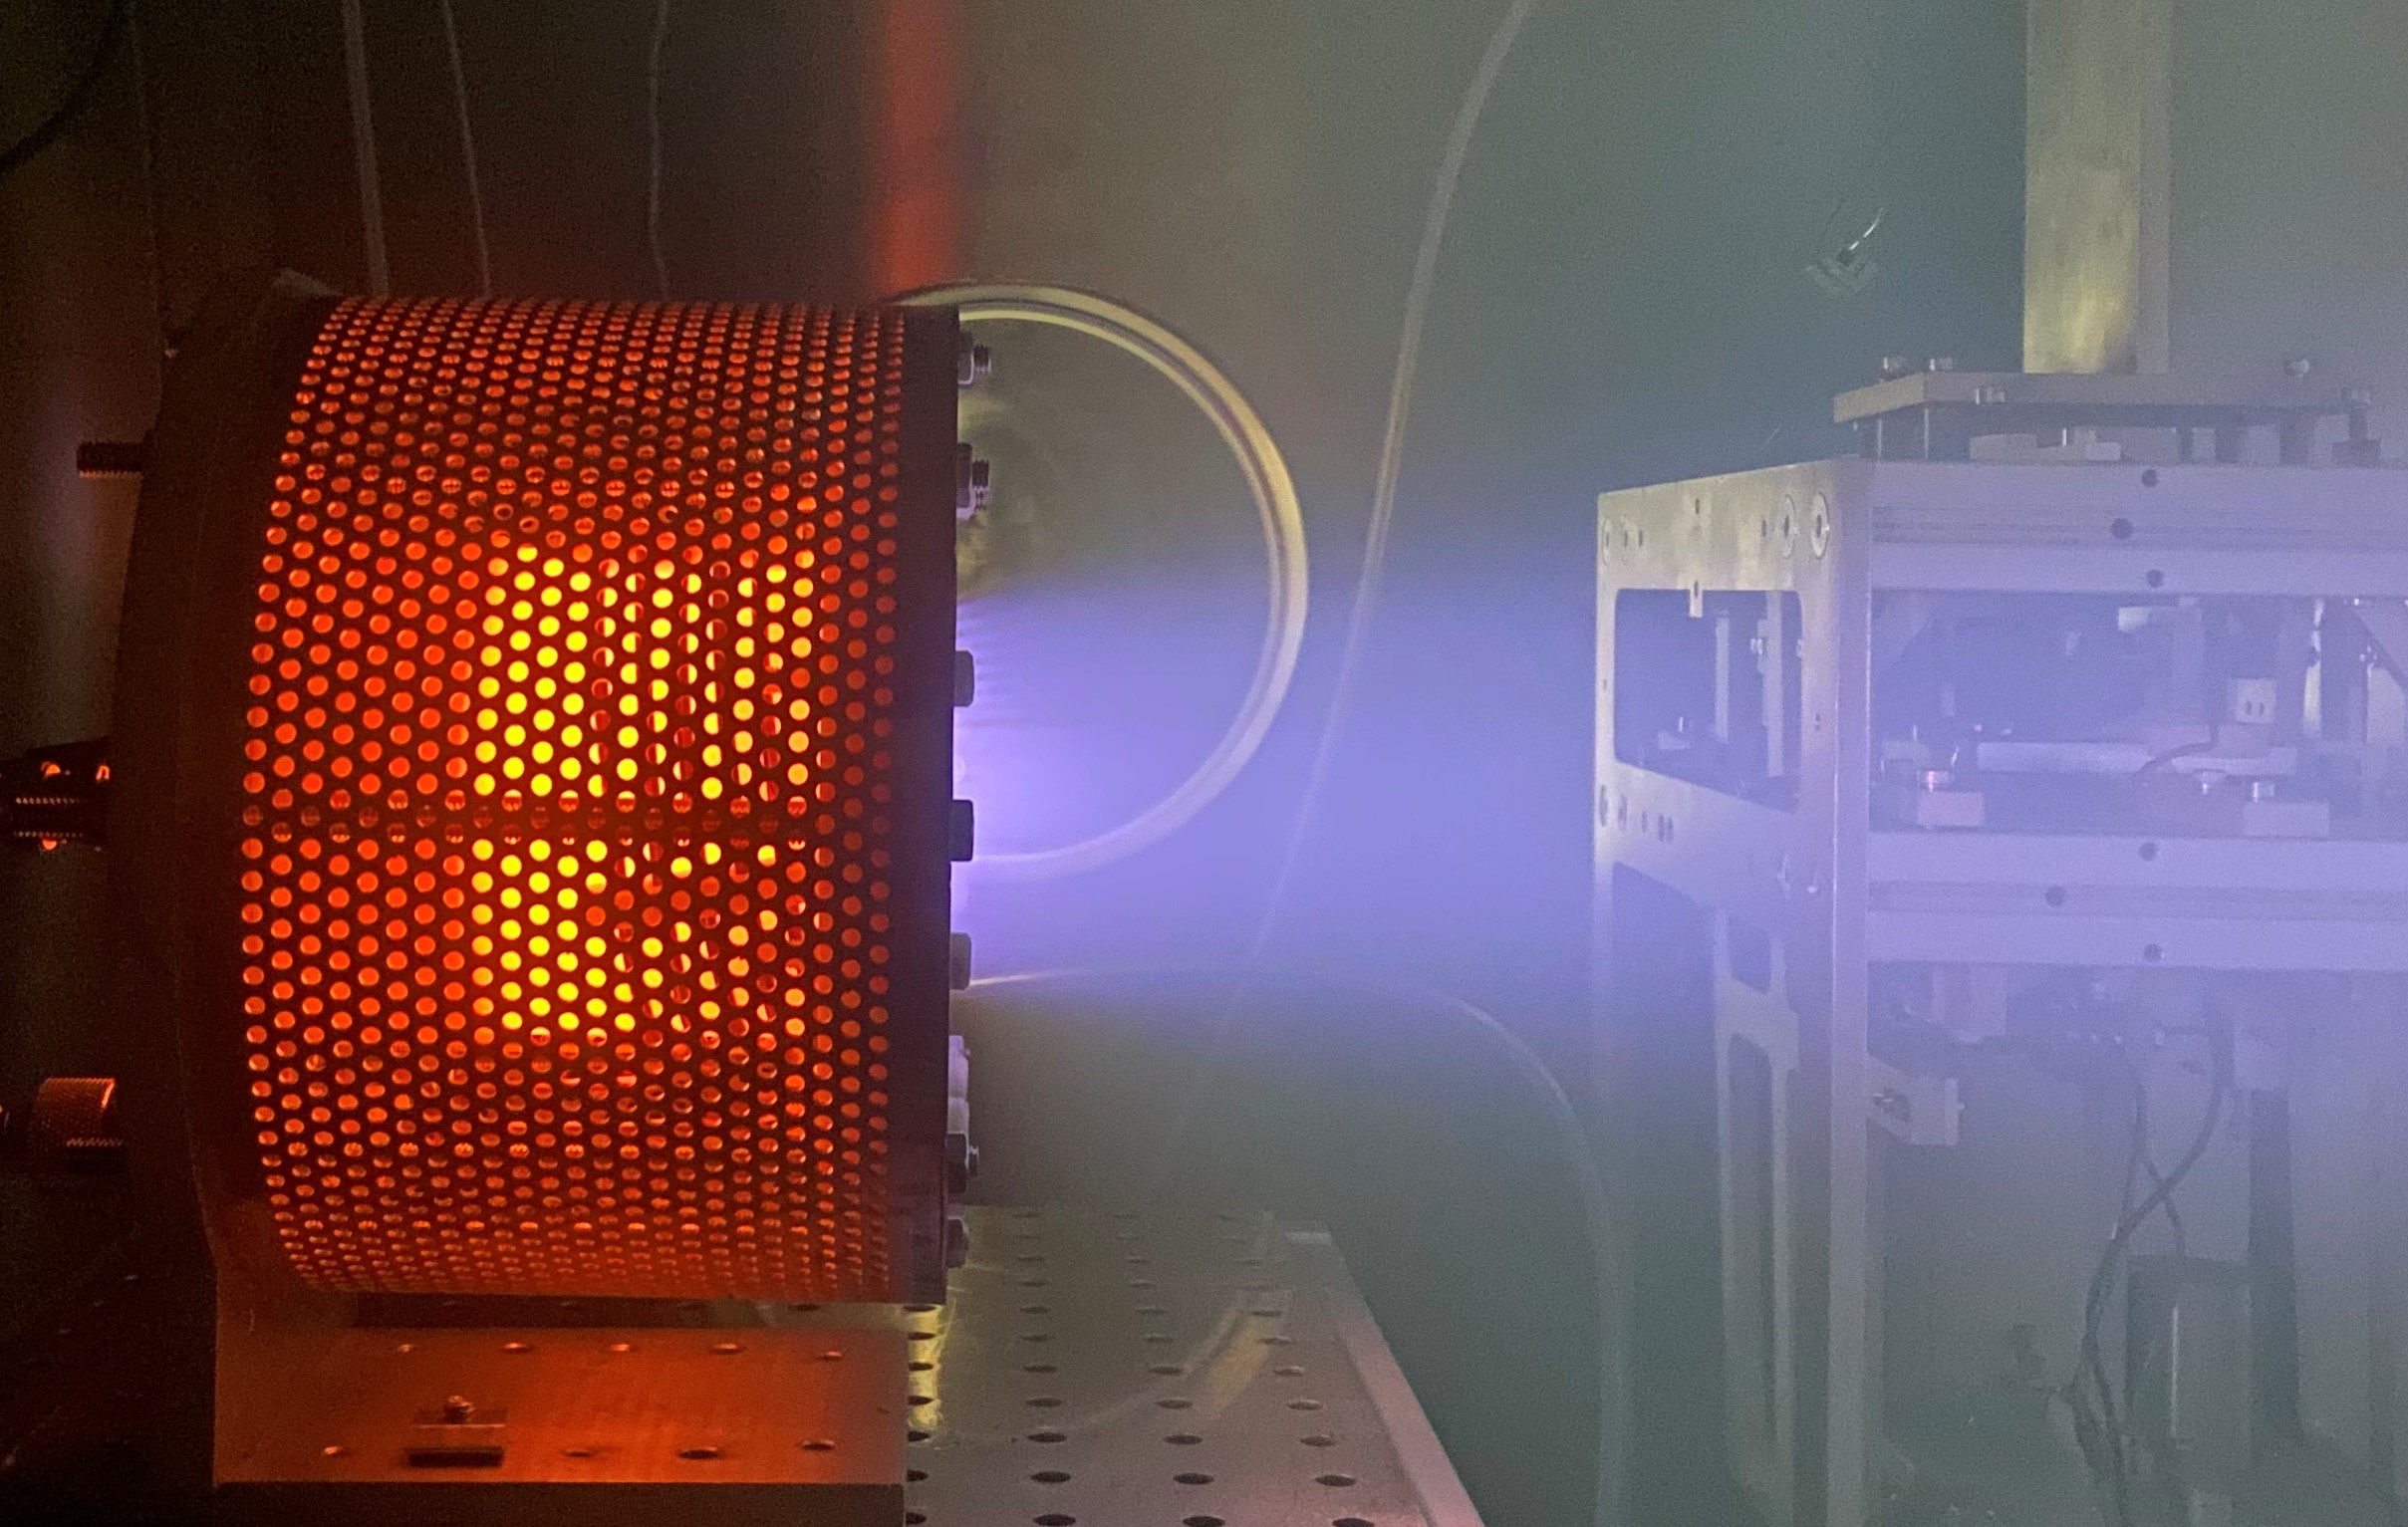
\includegraphics[scale=0.15]{fig/beamdiv.jpg}
\caption{Ion beam and divergence of BURFIT-80}
\label{fig:beamdivergence2}
\end{figure}

In figure \ref{fig:beamdivergence2} it can be clearly seen that beam originating from the thruster is dispersing in a direction perpendicular to the thruster axis. In order to include a correction factor for thrust calculations following formula is introduced. 

\begin{equation}
    F_t = cos\theta
    \label{eq:divergenceangle}
\end{equation}

Second factor to consider in thrust calculations is the ratio of doubly charged ions to singly charged ions. Electron with a sufficient energy can collide with an already ionized particle
and can release a second electron, creating a doubly ionized particle. Doubly ionized particles require more energy to ionize and consume the kinetic energy which could be otherwise be used to singly-ionize other particles. In order to account for this energy loss coefficient $\alpha$ is introduced. It is defined as\cite{goebel2008fundamentals};

\begin{equation}
    \alpha = \frac{I^+ + \dfrac{1}{\sqrt{2}I^{++}}}{I^+ + I^{++}} =  \frac{1+0.707\dfrac{I^{++}}{I+}}{1+\dfrac{I^{++}}{I^+}}
    \label{eq:alpha}
\end{equation}

where $I^+$ and $I^{++}$ are singly charged ion and doubly charged ion current respectively. Combining both correction factors from equations \ref{eq:divergenceangle} and \ref{eq:alpha} gives thrust correction coefficient $\gamma$;

\begin{equation}
    \gamma = \alpha F_t 
    \label{eq:gamma}
\end{equation}

Subsequently thrust formula from equation \ref{eq:uncorrectedthrust} turns into;

\begin{equation}
    T = \gamma \sqrt{\dfrac{2m_i V_b}{e}}I_b
    \label{eq:correctedthrust}
\end{equation}

Equation \ref{eq:correctedthrust} will be used to calculate thrust levels of designed prototype in chapter \ref{ch:Ch3}.

\subsection{Specific Impulse}
As mentioned earlier in chapter \ref{purposeofthesis} specific impulse is a measure to assess the thrusters propellant usage efficiency. It is defined as\cite{goebel2008fundamentals};
\begin{equation}
    I_{sp} = \frac{T}{\dot{m}_p g}
    \label{eq:specimpulse}
\end{equation}

Substituting the T expression from equation \ref{eq:momentumchange} gives;

\begin{equation}
    I_{sp} = \frac{v_{ex}}{g}
    \label{eq:specimpulse2}
\end{equation}

Substituting equation \ref{eq:epthrust} for $v_{ex}$ gives;

\begin{equation}
    I_{sp} = \frac{v_i}{g}\frac{\dot{m}_i}{\dot{m}_p}
    \label{eq:specimpulse3}
\end{equation}

in which the part $\dfrac{\dot{m}_i}{\dot{m}_p}$, ratio of ionized propellant to non-ionized propellant is defined as mass utilization efficiency $\eta_m$.

\begin{equation}
    I_{sp} = \frac{v_i}{g}\eta_m
    \label{eq:specimpulse4}
\end{equation}

Using equation \ref{eq:ionvel2} for ion velocity and adding correction factor $\gamma$ to account for correction factors as in thrust calculations gives;

\begin{equation}
    I_{sp} = \frac{\eta_m}{g}\sqrt{\frac{2e V_b}{I_b}}
    \label{eq:specimpulse5}
\end{equation}

Equation \ref{eq:specimpulse5} will be used to calculate specific impulse values in chapter \ref{ch:Ch3}.

% \subsection{RF System Design}
% \subsection{Power Consumption}
% \subsection{Efficiency}
\subsection{Neutralizer}
As the thruster fires positively charged ions will rapidly leave the thruster which will cause the spacecraft to be negatively charged. This situation is undesirable since loss of spacecraft's electrical ground will inevitably cause other subsystems of the spacecraft to stop properly functioning. Also positively charged particles in the ion beam can backstream into the thruster itself or adhere themselves to other sensitive surfaces of the spacecraft.  In order to compensate for this imbalanced load a neutralizer is placed in such position that emitted electrons will neutralize the ion beam. This neutralizer can be a complex system such as hollow cathode, shown in figure \ref{fig:burfitneut} or can be simple such as a tungten filament, shown in figure \ref{fig:tungstenneut}. 

\begin{figure}[ht]
    \centering
    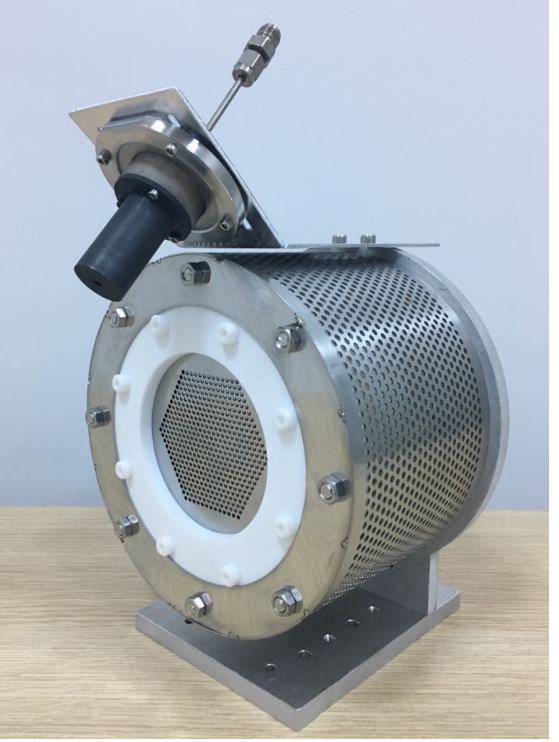
\includegraphics[scale=0.5]{fig/burfitneut.png}
    \caption[BURFIT-80 with neutralizer hollow cathode attached on top]{BURFIT-80 with neutralizer hollow cathode attached on top\cite{kokal2019development}}
    \label{fig:burfitneut}  
\end{figure}

\begin{figure}[ht]
    \centering
    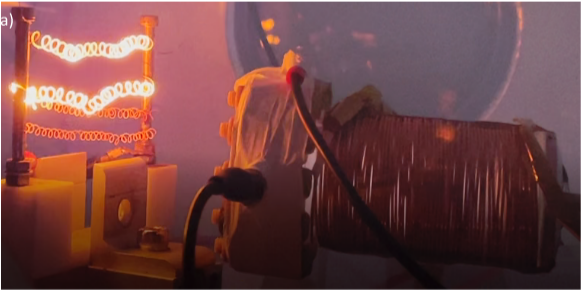
\includegraphics[scale=0.75]{fig/tungstenneut.png}
    \caption{Thruster operation with tungsten filament placed at ion beam downstream(\textbf{ATIF YAYINLANMADI})}
    \label{fig:tungstenneut}  
\end{figure}

Although a neutralizer is essential for space operations, in this work it is not included. This is because testing is conducted in a vacuum chamber that has its wall grounded, effectively
negating the need for an external neutralizer. 

% Tables and figures given in appendices must be numbered with the number of the appendix they are in (i.e. Table \ref{TableA.1}, Table A.2, Figure A.1, Figure A.2).

% In tables and figures, font size could be reduced to 8 pt, if necessary.

% Tables must be prepared using the same font type as the thesis. The font type used in figures must be consistent throughout the thesis.

% Tables and figures must be placed after they are first cited in the main text body, but must be as close as possible, in accordance with the rules in this guideline (Figure \ref{Figure2.1}). All tables and figures must be cited before they are used in the main text body (Table \ref{Table2.1}).

% All tables and figures must be horizontally centered on the page.

% The numbering of the tables and the figures must be such that the first number is the number of the chapter the table/figure is placed under (for appendices, the letter of the appendix), and the second number is the number of order (i.e. Table \ref{Table2.2}, Figure \ref{Figure2.2}, Table \ref{TableA.1}, Figure \ref{Figure2.3}). The words “Table” and “Figure” and numbers must be bold.

% For table numbers and captions, 1 line spacing, 12 pt (before) and 6 pt (after) paragraph spacing must be set. Table captions must be ended with a full stop. A table and its caption must be on the same page. 

% Multiple tables/figures could be placed on one page, however, table/figures spanning more than 4 consecutive pages must be given in appendices rather than the main text body.

% The first paragraph following a table must have 12 pt (before) and 6 pt (after) paragraph spacing. Titles following a table must have the standard formatting as previously specified. 

% Footnotes for a table must be written with 1 line spacing and a font size 2 pt smaller than the main text body. 
% For figure numbers and captions, 1 line spacing, 6 pt (before) and 12 pt (after) paragraph spacing must be set. Figure captions must be ended with a full stop. A figure and its caption must be on the same page. 

% For figures spanning more than one page, the same number and caption must be written below the continued figure, with the expression ”continued” added in brackets (i.e. \textbf{Table \ref{Table2.1} (continued):} Metal composition of wastes. \textbf{Figure \ref{Figure2.1} (continued):} Water supply network of ISTANBUL.).

% Plots, images and musical notes must be numbered and captioned as figures. Musical notes must be written according to the format rules set by the ITU School of Traditional Turkish Music. 

% It is recommended that elements that increase the page thickness and disrupt the binding structure of theses such as  folded pages or additional items embedded on pages are given as appendices.

% \vspace{6pt}
% \begin{figure}[h]
% 	\centering
% 	
\includegraphics[scale=.3]{./fig/sekil1}
% 	% sekil1.eps: 0x0 pixel, 300dpi, 0.00x0.00 cm, bb=14 14 592 479
% 	\vspace{6pt}
% 	\caption{All tables and figures must be horizontally centered on the page.}
% 	\label{Figure2.1}
% \end{figure}

%\begin{figure}
%	\begin{minipage}[b]{.5\linewidth}
%		\centering
%		
\includegraphics[scale=.2]{./fig/sekil1}
%		\subcaption{A subfigure}\label{Figure2.2a}
%	\end{minipage}
%	\begin{minipage}[b]{.5\linewidth}
%		\centering
%		
\includegraphics[scale=.2]{./fig/sekil1}
%		\subcaption{Another subfigure}\label{Figure2.2b}
%	\end{minipage}
%	\caption{A figure}\label{Figure2.2} % If no need a caption for main figure comment it out 
%\end{figure}
%%Figure letter: \subref{Figure2.2a}

%\begin{figure}
%	\begin{subfigure}[b]{.5\linewidth}
%		\centering
%		
\includegraphics[scale=.2]{./fig/sekil1}
%		\caption{A subfigure}\label{Figure2.3a}
%	\end{subfigure}
%	\begin{subfigure}[b]{.5\linewidth}
%		\centering
%		
\includegraphics[scale=.2]{./fig/sekil1}
%		\caption{Another subfigure}\label{Figure2.3b}
%	\end{subfigure}
%	\caption{A figure}\label{Figure2.3}
%\end{figure}

% Subfigure example with proper LOF usage - SBÖ
% \begin{figure}[h]
% 	\centering
% 	\begin{subfigure}{.8\textwidth}
% 		\centering
% 		
\includegraphics[scale=.3]{./fig/sekil1}
% 		\firstsubcaption{First subcaption of the subfigure.}
% 		\label{Figure2.2a}
% 	\end{subfigure}
% 	\begin{subfigure}{.8\textwidth}
% 		\centering
% 		
\includegraphics[scale=.3]{./fig/sekil1}
% 		\nextsubcaption{Second subcaption of the subfigure.}
% 		\label{Figure2.2b}
% 	\end{subfigure}
%     \caption{An example of subfigure main caption.}\label{Figure2.2}
% \end{figure}

%\begin{figure}
%	\centering     % not \center
%	\subcaption[]{Another subfigure}{\label{fig:a}
\includegraphics[scale=.2]{./fig/sekil1}}
%	\subcaption[]{Another subfigure}{\label{fig:b}
\includegraphics[scale=.2]{./fig/sekil1}}
%	%\caption{(a) this is fig 1 (b) this is fig 2.}
%	\label{L50}
%\end{figure}

% In Figure \ref{Figure2.2}, sed diam nonumy eirmod tempor invidunt ut labore et dolore magna aliquyam erat, sed diam voluptua. At vero eos et accusam et justo duo dolores et ea rebum. Lorem ipsum dolor sit amet, consetetur sadipscing elitr, sed diam nonumy eirmod tempor invidunt ut labore et dolore magna aliquyam erat, sed diam voluptua. At vero eos et accusam et justo duo dolores et ea rebum. At vero eos et accusam et justo duo dolores et ea rebum. At vero eos et accusam et justo duo dolores et ea rebum. At vero eos et accusam et justo duo dolores et ea rebum. At vero eos et accusam et justo duo dolores et ea rebum. At vero eos et accusam et justo duo dolores et ea rebum. At vero eos et accusam et justo duo dolores et ea rebum in Figure \ref{Figure2.2a}.

% \begin{figure}
% 	\centering
% 	
\includegraphics[width=10cm,keepaspectratio=true]{./fig/sekil2}
% 	% sekil2.eps: 0x0 pixel, 300dpi, 0.00x0.00 cm, bb=14 14 818 556
% 	\vspace{3pt}
% 	\caption{Example figure.}
% 	\label{Figure2.3}
% \end{figure}
% \vspace{-6pt}
% \section{Landscape-oriented, full-page figure}


% % Change margins on the fly to reset the page margins to one inch - SBÖ
% \newenvironment{changemargin}[4]{
% 	\begin{list}{}{
% 			\setlength{\voffset}{#1}
% 			\setlength{\oddsidemargin}{#2}
% 			\setlength{\evensidemargin}{#3}
% 			\setlength{\textheight}{#3}
% 		}
% 		\item[] ~ \par
% 		% Get rid of the extra space inserted by the previous line
% 		%\vspace*{-2em}
% 	}{
% 	\end{list}
% }

% % All the figures and also odd page figures normally face inside the thesis, however the rule requires figures always face to the right. - SBÖ
% % Figures on landscape pages has to be centered and facing to the right (ITU) - SBÖ
% \begin{landscape}
% 	\thispagestyle{empty} %Remove the bottom page numbering
% %	\begin{changemargin}{-0.4mm}{0mm}{0mm} %Set all the margins to zero - SBÖ
% 	%\thispagestyle{lscape}
% 	\vspace*{5mm}
% 	\begin{figure*}[ht]
% 		\centering
% 		%\begin{tabular}{@{}cc@{}}
% 		
\includegraphics[scale=.41,keepaspectratio=true]{./fig/sekil3} %&
% 		%
\includegraphics[width=50mm]{./fig/sekil3}
% 		%\end{tabular}                                       
% 		\caption{Landscape-oriented, full-page figure.}
% 		\label{Figure2.4}
% 	\end{figure*}
	
% % Set the page number on the right side for odd numbered pages
%       \begin{tikzpicture}[remember picture, overlay]
% 		\node[xshift=-25mm+148.5mm, yshift=17mm-210mm+15mm] (number) at (current page text area.east) {\thepage};
% 	  \end{tikzpicture}
	  
% %\end{changemargin}
% \end{landscape}

% % All the figures and also even page figures normally face inside the thesis, however the rule requires figures always face to the right. - SBÖ
% % Figures on landscape pages has to be centered and facing to the right (ITU) - SBÖ
% \begin{landscape}
% 	\thispagestyle{empty} % Remove the bottom page numbering
% %	\begin{changemargin}{-0.4mm}{0mm}{0mm} %Set all the margins to zero - SBÖ
% 		%\thispagestyle{lscape}

% 		\vspace*{20mm}
% 		\begin{figure*}[ht]
% 			\centering
% 			%\begin{tabular}{@{}cc@{}}
% 				
\includegraphics[scale=.41,keepaspectratio=true]{./fig/sekil3} %&
% 				%
\includegraphics[width=50mm]{./fig/sekil3}
% 			%\end{tabular}                                       
% 			\caption{Landscape-oriented, full-page figure.}
% 			\label{Figure2.5}
% 		\end{figure*}
	   
% % Set the page number on the left side for even numbered pages
% 		%\begin{tikzpicture}[remember picture, overlay]
% 		% \node[xshift=-25mm+148.5mm, yshift=-1mm-15mm, rotate=180] (number) at (current page text area.east) {\thepage};
% 		%\end{tikzpicture}
		
% % Set the page number on the right side for even numbered pages as well
% 		\begin{tikzpicture}[remember picture, overlay]
% 		 \node[xshift=-25mm+148.5mm, yshift=17mm-210mm] (number) at (current page text area.east) {\thepage};
% 		\end{tikzpicture}
		
% %	\end{changemargin}
% \end{landscape}

% %\newpage
% \section{Table Citations and Table Example}
% \begin{table*}[h]
% 	{\setlength{\tabcolsep}{14pt}
% 		\caption{Table with single row and centered columns.}
% 		\begin{center}
% 			\vspace{-6mm}
% 			\begin{tabular}{cccc}
% 				\hline \\[-2.45ex] \hline \\[-2.1ex]
% 				Column A & Column B & Column C & Column D \\
% 				\hline \\[-1.8ex]
% 				Row A & Row A & Row A & Row A \\
% 				Row B & Row B & Row B & Row B \\
% 				Row C & Row C & Row C & Row C \\
% 				\hline
% 			\end{tabular}
% 			\vspace{-6mm}
% 		\end{center}
% 		\label{Table2.1}}
% \end{table*}

% As seen in Table \ref{Table2.1}, 
% \begin{table*}[h]
% 	{\setlength{\tabcolsep}{14pt}
% 		\caption{Table captions must be ended with a full stop.}
% 		\begin{center}
% 			\vspace{-6mm}
% 			\begin{tabular}{cccc}
% 				\hline \\[-2.45ex] \hline \\[-2.1ex]
% 				Column A & Column B & Column C & Column D \\
% 				\hline \\[-1.8ex]
% 				Row A & Row A & Row A & Row A \\
% 				Row B & Row B & Row B & Row B \\
% 				Row C & Row C & Row C & Row C \\
% 				\hline
% 			\end{tabular}
% 			\vspace{-6mm}
% 		\end{center}
% 		\label{Table2.2}}
% \end{table*}



% \section{Landscape-oriented, full-page table}


% % ---------------------------------------------------------------- %
% % Page numbers must be on the bottom-middle of short side (when    %
% % portrait-oriented), or bottom-middle of long side (when	       %
% % landscape-oriented)						                       %
% % ---------------------------------------------------------------- %
% % Odd page landscape table and page numbering - SBÖ		
% \begin{landscape}
% 	\thispagestyle{empty}
% %	\vspace*{-6mm}
% %	\begin{changemargin}{0.4mm}{0mm}{0mm} %Set all the margins to zero - SBÖ
% 	\begin{table*}[htb!]
% 		{\setlength{\tabcolsep}{14pt}
% 			%\hspace*{5mm}
% 			%\vspace*{-6mm}
% 			\caption{Prof. Dr. Galip TEPEHAN \,\, Captioning in landscape-oriented pages:
% 				the most important aspect is to align the lines horizontally.}
% 			\begin{center}
% 				\vspace{-6mm}
% 				\begin{tabular}{lccrrrrr}
% 					\hline\hline
% 					\multirow{2}{*}{Parametre} & \multirow{2}{*}{Column 2} & \multirow{2}{*}{Column 3} & \multicolumn{3}{c|}{Column 4} & \multicolumn{2}{c}{Column 5}\\ \cline{4-8}
% 					& & & Subcolumn & Subcolumn & Subcolumn & Subcolumn & Subcolumn\\
% 					\hline
% 					Row 1 & -7.680442 & 7.6986348 & 0.00 & 0.00 & 0.00 & 12 & 12 \\
% 					Row 2 & 140 & - & 0.50 & 0.00 & 0.00 & 0 & 0 \\
% 					Row 3 & 37.174357 & 37.16192697 & 0.00 & 0.00 & 0.00 & 0 & 24 \\
% 					Row 4 & 140 & - & 0.50 & 0.00 & 0.00 & 0 & 0 \\
% 					Row 5 & 37.174357 & 37.16192697 & 0.00 & 0.00 & 0.00 & 0 & 24 \\
% 					Row 6 & 140 & - & 0.50 & 0.00 & 0.00 & 0 & 0 \\
% 					Row 7 & 37.174357 & 37.16192697 & 0.00 & 0.00 & 0.00 & 0 & 24 \\
% 					Row 8 & 140 & - & 0.50 & 0.00 & 0.00 & 0 & 0 \\
% 					Row 9 & 37.174357 & 37.16192697 & 0.00 & 0.00 & 0.00 & 0 & 24 \\
% 					Row 10 & 140 & - & 0.50 & 0.00 & 0.00 & 0 & 0 \\
% 					Row 11 & 37.174357 & 37.16192697 & 0.00 & 0.00 & 0.00 & 0 & 24 \\
% 					Row 12 & 140 & - & 0.50 & 0.00 & 0.00 & 0 & 0 \\
% 					Row 13 & 37.174357 & 37.16192697 & 0.00 & 0.00 & 0.00 & 0 & 24 \\
% 					Row 14 & 140 & - & 0.50 & 0.00 & 0.00 & 0 & 0 \\
% 					Row 15 & 37.174357 & 37.16192697 & 0.00 & 0.00 & 0.00 & 0 & 24 \\
% 					\hline
% 				\end{tabular}
% 			\end{center}
% 			\begin{center}
% 				\label{Table2.3}
% 			\end{center}
% 		}
% 	\end{table*}
% % Set the page number on the right side for odd numbered pages
% 		\begin{tikzpicture}[remember picture,overlay]
% 		\node[xshift=-10mm+148.5mm, yshift=2mm-210mm+30mm] (number) at (current page text area.east) {\thepage};
% 		\end{tikzpicture}
% %   \end{changemargin}
% \end{landscape}

% % ---------------------------------------------------------------- %
% % Page numbers must be on the bottom-middle of short side (when    %
% % portrait-oriented), or bottom-middle of long side (when	       %
% % landscape-oriented)						                       %
% % ---------------------------------------------------------------- %
% % Even page landscape table and page numbering - SBÖ		
% \begin{landscape}
% 	\thispagestyle{empty}
% 	%\vspace*{-6mm}
% %	\begin{changemargin}{0.4mm}{0mm}{0mm} %Set all the margins to zero - SBÖ
% 		\begin{table*}[htb!]
% 			{\setlength{\tabcolsep}{14pt}
% 				%\hspace*{5mm}
% 				%\vspace*{-6mm}
% 				\caption{Prof. Dr. Galip TEPEHAN \,\, Captioning in landscape-oriented pages:
% 					the most important aspect is to align the lines horizontally.}
% 				\begin{center}
% 					\vspace{-6mm}
% 					\begin{tabular}{lccrrrrr}
% 						\hline\hline
% 						\multirow{2}{*}{Parametre} & \multirow{2}{*}{Column 2} & \multirow{2}{*}{Column 3} & \multicolumn{3}{c|}{Column 4} & \multicolumn{2}{c}{Column 5}\\ \cline{4-8}
% 						& & & Subcolumn & Subcolumn & Subcolumn & Subcolumn & Subcolumn\\
% 						\hline
% 						Row 1 & -7.680442 & 7.6986348 & 0.00 & 0.00 & 0.00 & 12 & 12 \\
% 						Row 2 & 140 & - & 0.50 & 0.00 & 0.00 & 0 & 0 \\
% 						Row 3 & 37.174357 & 37.16192697 & 0.00 & 0.00 & 0.00 & 0 & 24 \\
% 						Row 4 & 140 & - & 0.50 & 0.00 & 0.00 & 0 & 0 \\
% 						Row 5 & 37.174357 & 37.16192697 & 0.00 & 0.00 & 0.00 & 0 & 24 \\
% 						Row 6 & 140 & - & 0.50 & 0.00 & 0.00 & 0 & 0 \\
% 						Row 7 & 37.174357 & 37.16192697 & 0.00 & 0.00 & 0.00 & 0 & 24 \\
% 						Row 8 & 140 & - & 0.50 & 0.00 & 0.00 & 0 & 0 \\
% 					\end{tabular}
% 				\end{center}
% 				\begin{center}
% 					\label{Table2.4}
% 				\end{center}
% 			}
% 		\end{table*}
% % Set the page number on the right side for even numbered pages
% 		\begin{tikzpicture}[remember picture,overlay]
% 		\node[xshift=-25mm+148.5mm, yshift=2mm-210mm+15mm] (number) at (current page text area.east) {\thepage};
% 		\end{tikzpicture}
% %	\end{changemargin}
% \end{landscape}

% \begin{table}[!htbp] \centering
% 	\caption{ Neighborhoods Visited }
% 	\vspace{-3mm}
% 	\label{}
% 	\begin{tabular}{@{\extracolsep{5pt}} llrrr} 
% 	\\[-1.8ex]\hline 
% 		\hline \\[-1.8ex] 
% 		\multicolumn{1}{c}{Variable} & \multicolumn{1}{c}{Values} & \multicolumn{1}{c}{Count} & \multicolumn{1}{c}{\%} & \multicolumn{1}{c}{Cum. \%} \\
% 		\hline \\[-1.8ex] 
% 		\multirow{ 4 }{*}{ visit }  &  FALSE  &  2  &  33.33  &  33.33  \\
% 		\hhline{}  &  TRUE  &  3  &  50.00  &  83.33  \\
% 		\hhline{}  &  NA  &  1  &  16.67  &  100.00  \\
% 	    \hhline{}  &  Total  &  6  &  100.00  &    \\
% 		\hline \\[-1.8ex] 
% 	\end{tabular}
% \end{table}

% % Multi-page longtable example spreading couple of pages - SBÖ
% \begin{center}
% 	\begin{longtable}{ccc}
% 		%Here is the caption, the stuff in [] is the table of contents entry,
% 		%the stuff in {} is the title that will appear on the first page of the
% 		%table.
% 		\caption[Feasible triples for a highly variable Grid]{Feasible triples
% 			for highly variable Grid, MLMMH.} \label{Table2.6} \vspace{-1.75mm}\\
% 		%This is the header for the first page of the table...
% 		\hline\\[-2.45ex] \hline \\[-1.8ex] % Distancing of the hlines adjausted from the text 
% 		\multicolumn{1}{c}{{Time (s)}} &
% 		\multicolumn{1}{c}{{Triple chosen}} &
% 		\multicolumn{1}{c}{{Other feasible triples}} \\[0.5ex] \hline
% 		\\[-1.8ex]
% 		\endfirsthead
		
% 		%This is the header for the remaining page(s) of the table...
% 		\multicolumn{3}{c}{{\tablename} \textbf{\thetable{}} \textbf{(continued) :} Feasible triples
% 			for highly variable Grid, MLMMH.} \\[0.5ex]
% 		\hline\\[-2.45ex] \hline \\[-1.8ex]
% 		\multicolumn{1}{c}{{Time (s)}} &
% 		\multicolumn{1}{c}{{Triple chosen}} &
% 		\multicolumn{1}{c}{{Other feasible triples}} \\[0.5ex] \hline
% 		\\[-1.8ex]
% 		\endhead
		
% 		%This is the footer for all pages except the last page of the table...
% 		%\multicolumn{3}{l}{{Continued on Next Page\ldots}} \\
% 		\\[-1.8ex] \hline
% 		\endfoot
		
% 		%This is the footer for the last page of the table...
% 		\\[-1.8ex] \hline
% 		\endlastfoot
		
% 		%Now the data...
% 		0      & (1, 11, 13725) & (1, 12, 10980), (1, 13, 8235), (2, 2, 0), (3, 1, 0) \\
% 		2745   & (1, 12, 10980) & (1, 13, 8235), (2, 2, 0), (2, 3, 0), (3, 1, 0) \\
% 		5490   & (1, 12, 13725) & (2, 2, 2745), (2, 3, 0), (3, 1, 0) \\
% 		8235   & (1, 12, 16470) & (1, 13, 13725), (2, 2, 2745), (2, 3, 0), (3, 1, 0) \\
% 		% <data removed>
% 		164700 & (1, 13, 13725) & (2, 2, 2745), (2, 3, 0), (3, 1, 0) \\
% 		0      & (1, 11, 13725) & (1, 12, 10980), (1, 13, 8235), (2, 2, 0), (3, 1, 0) \\
% 		2745   & (1, 12, 10980) & (1, 13, 8235), (2, 2, 0), (2, 3, 0), (3, 1, 0) \\
% 		5490   & (1, 12, 13725) & (2, 2, 2745), (2, 3, 0), (3, 1, 0) \\
% 		8235   & (1, 12, 16470) & (1, 13, 13725), (2, 2, 2745), (2, 3, 0), (3, 1, 0) \\
% 		% <data removed>
% 		164700 & (1, 13, 13725) & (2, 2, 2745), (2, 3, 0), (3, 1, 0) \\
% 		0      & (1, 11, 13725) & (1, 12, 10980), (1, 13, 8235), (2, 2, 0), (3, 1, 0) \\
% 		2745   & (1, 12, 10980) & (1, 13, 8235), (2, 2, 0), (2, 3, 0), (3, 1, 0) \\
% 		5490   & (1, 12, 13725) & (2, 2, 2745), (2, 3, 0), (3, 1, 0) \\
% 		8235   & (1, 12, 16470) & (1, 13, 13725), (2, 2, 2745), (2, 3, 0), (3, 1, 0) \\
% 		% <data removed>
% 		164700 & (1, 13, 13725) & (2, 2, 2745), (2, 3, 0), (3, 1, 0) \\
% 		0      & (1, 11, 13725) & (1, 12, 10980), (1, 13, 8235), (2, 2, 0), (3, 1, 0) \\
% 		2745   & (1, 12, 10980) & (1, 13, 8235), (2, 2, 0), (2, 3, 0), (3, 1, 0) \\
% 		5490   & (1, 12, 13725) & (2, 2, 2745), (2, 3, 0), (3, 1, 0) \\
% 		8235   & (1, 12, 16470) & (1, 13, 13725), (2, 2, 2745), (2, 3, 0), (3, 1, 0) \\
% 		% <data removed>
% 		164700 & (1, 13, 13725) & (2, 2, 2745), (2, 3, 0), (3, 1, 0) \\
% 		0      & (1, 11, 13725) & (1, 12, 10980), (1, 13, 8235), (2, 2, 0), (3, 1, 0) \\
% 		2745   & (1, 12, 10980) & (1, 13, 8235), (2, 2, 0), (2, 3, 0), (3, 1, 0) \\
% 		5490   & (1, 12, 13725) & (2, 2, 2745), (2, 3, 0), (3, 1, 0) \\
% 		8235   & (1, 12, 16470) & (1, 13, 13725), (2, 2, 2745), (2, 3, 0), (3, 1, 0) \\
% 		% <data removed>
% 		164700 & (1, 13, 13725) & (2, 2, 2745), (2, 3, 0), (3, 1, 0) \\
% 		0      & (1, 11, 13725) & (1, 12, 10980), (1, 13, 8235), (2, 2, 0), (3, 1, 0) \\
% 		2745   & (1, 12, 10980) & (1, 13, 8235), (2, 2, 0), (2, 3, 0), (3, 1, 0) \\
% 		5490   & (1, 12, 13725) & (2, 2, 2745), (2, 3, 0), (3, 1, 0) \\
% 		8235   & (1, 12, 16470) & (1, 13, 13725), (2, 2, 2745), (2, 3, 0), (3, 1, 0) \\
% 		% <data removed>
% 		164700 & (1, 13, 13725) & (2, 2, 2745), (2, 3, 0), (3, 1, 0) \\
% 		0      & (1, 11, 13725) & (1, 12, 10980), (1, 13, 8235), (2, 2, 0), (3, 1, 0) \\
% 		2745   & (1, 12, 10980) & (1, 13, 8235), (2, 2, 0), (2, 3, 0), (3, 1, 0) \\
% 		5490   & (1, 12, 13725) & (2, 2, 2745), (2, 3, 0), (3, 1, 0) \\
% 		8235   & (1, 12, 16470) & (1, 13, 13725), (2, 2, 2745), (2, 3, 0), (3, 1, 0) \\ \noalign{\penalty-5000}
% 		% <data removed>
% 		164700 & (1, 13, 13725) & (2, 2, 2745), (2, 3, 0), (3, 1, 0) \\
% 		0      & (1, 11, 13725) & (1, 12, 10980), (1, 13, 8235), (2, 2, 0), (3, 1, 0) \\
% 		2745   & (1, 12, 10980) & (1, 13, 8235), (2, 2, 0), (2, 3, 0), (3, 1, 0) \\
% 		5490   & (1, 12, 13725) & (2, 2, 2745), (2, 3, 0), (3, 1, 0) \\
% 		8235   & (1, 12, 16470) & (1, 13, 13725), (2, 2, 2745), (2, 3, 0), (3, 1, 0) \\
% 		% <data removed>
% 		164700 & (1, 13, 13725) & (2, 2, 2745), (2, 3, 0), (3, 1, 0) \\
% 		0      & (1, 11, 13725) & (1, 12, 10980), (1, 13, 8235), (2, 2, 0), (3, 1, 0) \\
% 		2745   & (1, 12, 10980) & (1, 13, 8235), (2, 2, 0), (2, 3, 0), (3, 1, 0) \\
% 		5490   & (1, 12, 13725) & (2, 2, 2745), (2, 3, 0), (3, 1, 0) \\
% 		8235   & (1, 12, 16470) & (1, 13, 13725), (2, 2, 2745), (2, 3, 0), (3, 1, 0) \\
% 		% <data removed>
% 		164700 & (1, 13, 13725) & (2, 2, 2745), (2, 3, 0), (3, 1, 0) \\
% 		0      & (1, 11, 13725) & (1, 12, 10980), (1, 13, 8235), (2, 2, 0), (3, 1, 0) \\
% 		2745   & (1, 12, 10980) & (1, 13, 8235), (2, 2, 0), (2, 3, 0), (3, 1, 0) \\
% 		5490   & (1, 12, 13725) & (2, 2, 2745), (2, 3, 0), (3, 1, 0) \\
% 		8235   & (1, 12, 16470) & (1, 13, 13725), (2, 2, 2745), (2, 3, 0), (3, 1, 0) \\
% 		% <data removed>
% 		164700 & (1, 13, 13725) & (2, 2, 2745), (2, 3, 0), (3, 1, 0) \\
% 		0      & (1, 11, 13725) & (1, 12, 10980), (1, 13, 8235), (2, 2, 0), (3, 1, 0) \\
% 		2745   & (1, 12, 10980) & (1, 13, 8235), (2, 2, 0), (2, 3, 0), (3, 1, 0) \\
% 		5490   & (1, 12, 13725) & (2, 2, 2745), (2, 3, 0), (3, 1, 0) \\
% 		8235   & (1, 12, 16470) & (1, 13, 13725), (2, 2, 2745), (2, 3, 0), (3, 1, 0) \\
% 		% <data removed>
% 		164700 & (1, 13, 13725) & (2, 2, 2745), (2, 3, 0), (3, 1, 0) \\
% 		0      & (1, 11, 13725) & (1, 12, 10980), (1, 13, 8235), (2, 2, 0), (3, 1, 0) \\
% 		2745   & (1, 12, 10980) & (1, 13, 8235), (2, 2, 0), (2, 3, 0), (3, 1, 0) \\
% 		5490   & (1, 12, 13725) & (2, 2, 2745), (2, 3, 0), (3, 1, 0) \\
% 		8235   & (1, 12, 16470) & (1, 13, 13725), (2, 2, 2745), (2, 3, 0), (3, 1, 0) \\
% 		% <data removed>
% 		164700 & (1, 13, 13725) & (2, 2, 2745), (2, 3, 0), (3, 1, 0) \\
% 		0      & (1, 11, 13725) & (1, 12, 10980), (1, 13, 8235), (2, 2, 0), (3, 1, 0) \\
% 		2745   & (1, 12, 10980) & (1, 13, 8235), (2, 2, 0), (2, 3, 0), (3, 1, 0) \\
% 		5490   & (1, 12, 13725) & (2, 2, 2745), (2, 3, 0), (3, 1, 0) \\
% 		8235   & (1, 12, 16470) & (1, 13, 13725), (2, 2, 2745), (2, 3, 0), (3, 1, 0) \\
% 	\end{longtable}
% \end{center}